% vim: set tw=72 spell spelllang=da:
\documentclass[a4paper, 10pt, danish, final]{report}
%%%%%%%%%%%%%%%%%%%%%%%%%%%%%%%%%%%%%%%%%%%%%%%%%%%%%%%%%%%%%%%%%
% Pakker
%%%%%%%%%%%%%%%%%%%%%%%%%%%%%%%%%%%%%%%%%%%%%%%%%%%%%%%%%%%%%%%%%
%\usepackage{a4wide}
\usepackage[danish]{babel}
\usepackage[utf8]{inputenc}
\usepackage[T1]{fontenc}

\usepackage{charter}
\usepackage{verbatim}
\usepackage{amsfonts}
\usepackage{amsmath}
\usepackage{amssymb}
%\usepackage{mathrsfs}
%\usepackage[mathcal]{euscript}
\usepackage{listings}
\usepackage{graphicx}
\usepackage{multirow}
\usepackage{hyperref}
\usepackage{cite}
\usepackage{float}
\usepackage[small,bf]{caption}
\usepackage{xypic}
\usepackage[table]{xcolor}
\usepackage{subfig}

%%%%%%%%%%%%%%%%%%%%%%%%%%%%%%%%%%%%%%%%%%%%%%%%%%%%%%%%%%%%%%%%
% Indstillinger
%%%%%%%%%%%%%%%%%%%%%%%%%%%%%%%%%%%%%%%%%%%%%%%%%%%%%%%%%%%%%%%%
\parindent=5pt
\lstset{language=Python, basicstyle=\scriptsize, showstringspaces=false, numbers=none, stepnumber=1, numberstyle=\tiny}
\setcounter{tocdepth}{1}

%%%%%%%%%%%%%%%%%%%%%%%%%%%%%%%%%%%%%%%%%%%%%%%%%%%%%%%%%%%%%%%%
% Kommandoer
%%%%%%%%%%%%%%%%%%%%%%%%%%%%%%%%%%%%%%%%%%%%%%%%%%%%%%%%%%%%%%%%
%\newcommand{\old}[1]{\oldstylenums{#1}}
%\newcommand{\old}[1]{{#1}}
\newcommand{\mailto}[1]{\href{mailto:#1}{#1}}
\newcommand{\resume}[1]{\begin{abstract}{\sffamily #1}\end{abstract}}
%\renewcommand{\thefigure}{\thechapter.\thesection.\arabic{figure}}
%\renewcommand{\thetable}{\thechapter.\thesection.\arabic{table}}

%%%%%%%%%%%%%%%%%%%%%%%%%%%%%%%%%%%%%%%%%%%%%%%%%%%%%%%%%%%%%%%
% Titel, forfatter og dato
%%%%%%%%%%%%%%%%%%%%%%%%%%%%%%%%%%%%%%%%%%%%%%%%%%%%%%%%%%%%%%%
\title{Detektion af ``Det Gyldne Snit'' i digitaliserede malerier}

\author{Ulrik Bonde - \mailto{bonde@diku.dk}\\
Kasper Steenstrup - \mailto{khsj@diku.dk}\\
Morten Thorlund - \mailto{thorlund@diku.dk}\\
\\
Vejleder\\Jakob Grue Simonsen}
\date{\today}

\hypersetup{
colorlinks,%
citecolor=black,%
filecolor=black,%
linkcolor=black,%
urlcolor=black,%
bookmarksopen=false,
pdftitle={Detektion af Det Gyldne Snit i digitaliserede malerier},
pdfauthor={Ulrik Bonde, Kasper Steenstrup og Morten Thorlund},
pdfsubject={Computer Vision},
pdfkeywords={Det gyldne snit, computer vision}
}

%%%%%%%%%%%%%%%%%%%%%%%%%%%%%%%%%%%%%%%%%%%%%%%%%%%%%%%%%%%%%%
% Indhold
%%%%%%%%%%%%%%%%%%%%%%%%%%%%%%%%%%%%%%%%%%%%%%%%%%%%%%%%%%%%%%
\begin{document}
\maketitle
\pagenumbering{roman}
\thispagestyle{empty}
%\pagestyle{headings}
\resume{
Det er den generelle opfattelse, at det gyldne snit er specielt æstetisk
tiltalende, og at det derfor er at finde i mange kunstmalerier.
Litteraturen kan ikke entydigt bekræfte denne påstand og den største
undersøgelse på området talte 565 malerier.  Selvom der findes metoder
fra billedbehandling, til systematisk analyse af billeders komposition,
er disse endnu ikke blevet taget i brug, med henblik på at undersøge
hypotesen om det gyldne snit.

Vi har udviklet et program som kan afgøre, hvorvidt en digital
gengivelse af et maleri, har interessante regioner liggende i det gyldne
snit, og kørt dette program på 17,364 digitale billeder af malerier.
Med vores metoder til udtrækning af regioner og to forskellige metoder
til vurdering af disse, kan vi ikke afvise, at det gyldne snit er
specielt æstetisk tiltalende. Ved naiv vurdering, viste hele
$\mathsf{91.43\%}$, af de analyserede malerier sig, at have én eller
flere regioner liggende i det gyldne snit. Resultaterne viser dog ingen
umiddelbar indikation på, at det gyldne snit adskiller sig signifikant
fra andre snit i malerier. Der vises nærmere en tendens til at kunstnere
foretrækker at placere interessante regioner i midten, mens den øverste
halvdel og kanterne af maleriet ikke er at foretrække.

%Resultaterne fra
%analysen opbevares i en database, som tillader videre arbejde med data.
%Programmet kan desuden analysere andre snit i billedet end blot det
%gyldne, og det bliver således muligt at skelne mellem og sammenligne
%resultater fra andre snit --- f.eks, kan vi skelne mellem resultater for
%det gyldne snit og for snit ved to tredjedele.

%Vi har udviklet et program, som kan trække sammenhængende regioner i
%nærheden af det gyldne snit, ud af en digital gengivelse af et maleri.
%Disse tages derefter ud og vurderes efter nogle simple kriterier for at
%afgøre, om de ligger i det gyldne snit. En automatisering af denne
%analyse er blevet sammensat, hvor en database gemmer resultaterne som
%tillader videre arbejde med data. Programmet kan desuden analysere andre
%snit i billedet end blot det gyldne, og det bliver således muligt at
%skelne mellem og sammenligne resultater fra forskellige snit --- f.eks,
%vil man kunne skelne mellem resultater for det gyldene snit og for snit
%ved en tredjedel.

}

{
\section*{Diff}
\begin{itemize}
	\item Reformulering og opstramning af afsnit om den naive
		algoritme (afsnit 3.4).\\
		Hovedpointer
		\begin{itemize}
			\item Regioner kan ligge i det gyldne snit
			\item Regioner kan være interessante
			\item Et billede opfylder det gyldne snit hvis
				det har mindst én interessant region der
				ligger i det gyldne snit.
		\end{itemize}
	\item Vi er blevet i tvivl om vores margin. Vi opererer sådan
		set med to. Et til bedre at kunne finde regioner med
		floodfill og et hvori vi vil acceptere regioner. Vi har
		endnu ikke fået regnet ordentligt igennem hvor stort det
		accepterende rektangel skal være.
\end{itemize}

}

% vim: set tw=72 spell spelllang=da:


% vim: set tw=72 spell spelllang=da:


\chapter*{Forord}
\addcontentsline{toc}{chapter}{Forord}
{
{\sffamily Dette dokument er den endelige rapport udarbejdet i forbindelse med
kurset ``Bachelorprojekt'' som udbydes på Datalogisk Institut ved
Københavns Universitet. Det forventes at læseren har en basal viden
inden for datalogi og kendskab til begreber der bruges i forbindelse med
billedbehandling.
}
}

%\subsection{Forventninger til læser} Dette opgave omhandler metoder og
%udledninger af akademiske problemer som opstår ved programmering inde for
%feltet billedbehandling, Derfor regner vi med at læseren af denne rapport har
%en basal vide inde for datalogi i retninger af billeders opbygning, det vil
%siger, viden om hvad en pixel er, hvad betjener RGB favre, osv. Dog ligger der
%vægt på at forklaring af vores problemer, Det vi er kommet frem til og hvad man
%kan bruge vores fund til. Ligger på en nivo som en kunst studerende kan
%relatere sig til og forstå.  Vi har tænkt på at lave en lille under afsnit til
%vær del i vores opgave, som forklare det vi laver med meget udpenslet sprog.

% vim: set tw=72 spell spelllang=da:


\tableofcontents
%\listoftables
%\listoffigures

\parskip=8pt plus 2pt minus 4pt

\chapter{Indledning}
\pagenumbering{arabic}
{
\textsf{
Dette kapitel har til formål at give en introduktion til det gyldne snit,
både matematisk og historisk. Der kastes et blik på den forskning, der
allerede er blevet gjort på området, hvilke metoder der er blevet brugt
og de metoder, der er til rådighed for ny forskning.
}

\section{Det gyldne snit\label{section_gyldne_snit}}
{
Det vi kalder det gyldne snit, den gyldne ratio eller det guddommelige
forhold, blev allerede beskrevet i Euklids \emph{Elements} fra ca. 300
f.  Kr. som følger:
\begin{quote}
	\emph{``A straight line is said to have been cut in extreme
	and mean ratio when, as the whole line is to the greater
	segment, so is the greater to the less.''}\cite{heath1908thirteen}
\end{quote}

\begin{figure}[h!]
	\begin{center}
		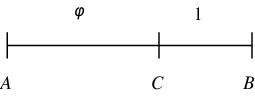
\includegraphics[scale=0.49,angle=0]{afsnit/baggrund/billeder/line_segment_a_c_b}
	\end{center}
	\caption{Euklids opdeling af et linjestykke}
	\label{line_segment}
\end{figure}

Givet et linjestykke $A\ B$, hvor $A\ B$ definerer linjen mellem
punkterne $A$ og $B$, som vist i figur \ref{euclid}, og ud fra Euklids
beskrivelse kan $\varphi$ defineres som
\begin{equation}
	\varphi	= \frac{A\ C}{C\ B} = \frac{A\ B}{A\ C}
	\label{euclid}
\end{equation}
Ved at indsætte variable i ligning \ref{euclid} får vi
\begin{equation}
	\varphi = \frac{\varphi + 1}{\varphi}
	\label{expand_euclid}
\end{equation}
hvilket giver os andengradsligningen
\begin{equation}
	\varphi^{2} - \varphi - 1 = 0.
	\label{poly_phi}
\end{equation}
Hvis vi nu løser andengradsligningen i \ref{poly_phi}, med
$\varphi > 0$, får vi
\begin{eqnarray*}
	\varphi	& =	& \frac{\sqrt{5} + 1}{2} \\
		& =	& 1.6180\ 3398\ 8749\ 8948\ 4820 \dots
\end{eqnarray*}

Tallet $\varphi$ bemærker sig blandt andet ved, at når det kvadreres, så
lægger man blot 1 til. Dette udledes trivielt fra ligning \ref{poly_phi}
\begin{equation}
	\varphi^{2} = \varphi + 1
	\label{phi_squared}
\end{equation}

Vi kan også finde polynomiets anden rod som angives ved $\varPhi$
\begin{eqnarray*}
	\varPhi & = & \frac{1}{\varphi} \\
		& = & \varphi - 1 \\
		& = & 0.6180\ 3398\ 8749\ 8948\ 4820 \dots
\end{eqnarray*}
Også tallet $\varPhi$ er interessant idet dets eget kvadrat plus sig
selv giver 1. Vi har at
\begin{equation}
	\varPhi^{2} + \varPhi = 1
	\label{Phi_squared}
\end{equation}
hvilket kun er gældende for $\varPhi$.

Tallet $\varphi$ fremviser endvidere en interessant forbindelse til
Fibonaccis talrække, da forholdet mellem to fibonaccital $F(n)$ og $F(n
- 1)$ konvergerer mod $\varphi$, når $n$ nærmer sig uendelig. Formelt har
vi at
\begin{eqnarray*}
	\varphi & =     & \lim_{n \rightarrow\infty}{\frac{F(n)}{F(n - 1)}}
\end{eqnarray*}

I tabel \ref{fibonacci_sequence} ses hvordan ratioen mellem fibonaccital
konvergerer mod $\varphi$, hvor også den procentvise afvigelse fra
$\varphi$ vises.

\begin{table}[h!]
    \centering
    \begin{tabular}{|c|c|c|c|c|}
        \hline
        $n$ & $F(n)$ & $F(n - 1)$ & $ \frac{F(n)}{F(n - 1)}$ & $\%$ fra $\varphi$ \\
        \hline
        0	 & 0 	 & $n/a$ & $n/a$ 		& $n/a$ 		\\
        1	 & 1	 & 1	 & 1.0		 	& 38.196601125 		\\
        2	 & 1	 & 1	 & 1.0		 	& 38.196601125 		\\
        3	 & 2	 & 1	 & 2.0		 	& -23.60679775 		\\
        4	 & 3	 & 2	 & 1.5			& 7.29490168752 	\\
        5	 & 5	 & 3	 & 1.66666666667	& -3.00566479165 	\\
        6	 & 8	 & 5	 & 1.6			& 1.11456180002 	\\
        7	 & 13	 & 8	 & 1.625	 	& -0.430523171858 	\\
        8	 & 21	 & 13	 & 1.61538461538	& 0.163740278863 	\\
        9	 & 34	 & 21	 & 1.61904761905	& -0.062645797602 	\\
        10	 & 55	 & 34	 & 1.61764705882	& 0.0239135845758 	\\
        11	 & 89	 & 55	 & 1.61818181818	& -0.00913636134662 	\\
        12	 & 144	 & 89	 & 1.61797752809	& 0.00348946069118 	\\
        13	 & 233	 & 144	 & 1.61805555556	& -0.00133290189271 	\\
        \hline
    \end{tabular}
    \caption{Fibonaccisekvens}
    \label{fibonacci_sequence}
\end{table}

\subsection{Et gyldent rektangel}
På samme måde som vi kan opdele et linjestykke efter det gyldne snit,
kan vi konstruere et rektangel, hvor forholdene mellem højde og bredde er
$\varphi$. Vi konstruerer et rektangel, hvor alle sider er lig 1, og
tegner en diagonal fra dette rektangels midte til dets modsatte hjørne. Med
denne diagonal som radius tegnes en cirkel, som et gyldent rektangel kan
tegnes efter. Figur \ref{golden_rectangle} illustrerer denne metode.

\begin{figure}[h!]
	\begin{center}
		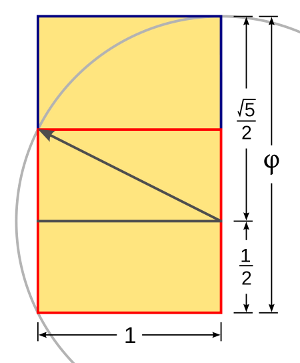
\includegraphics[scale=0.35,angle=0]{afsnit/baggrund/billeder/Golden_Rectangle_Construction}
	\end{center}
	\caption[Et gyldent rektangel]{Et gyldent rektangel - \emph{Kilde: Wikipedia}}
	\label{golden_rectangle}
\end{figure}
Det ses, at rektanglet har forholdet $\varphi:1$ og at eksemplet er helt
analogt til linjestykket givet i figur \ref{line_segment}. Dog skal
det bemærkes, at det rektangel, der kan konstrueres af linjestykkerne 1
og $\varphi - 1$, også er et gyldent rektangel med forholdet $1:\varphi
-1 = \varPhi$. Man kan derved konstruere gyldne rektangler ud i det
uendelige ved hele tiden at lave nye gyldne rektangler.

\subsection{Spiraler og det gyldne snit}
Når man, som ovenfor, gentagne gange deler et gyldent rektangel, kan man
bruge dette til at konstruere en gylden spiral. En gylden spiral kan
skrives ved ligningen for generelle logaritmiske spiraler som
\begin{equation}
	r = ae^{c\theta}
	\label{log_spiral_2}
\end{equation}
eller
\begin{equation}
	\theta = \frac{1}{c}\ln(r/a)
	\label{log_spiral_1}
\end{equation}
hvor $e$ er grundtallet for den naturlige logaritme og $c$ skal have en
speciel værdi for at kunne være en gylden spiral.

Det kan være svært at tegne logaritmiske spiraler korrekt, men man kan
approksimere en spiral ved at sammensætte dele af cirkler. Man kan
således approksimere en gylden spiral ved at sammensætte kvarte cirkler.
Denne approksimation giver dog ikke en ægte gylden spiral, og faktisk kan
ingen sådanne approksimationer af sammensatte cirkler gengives ved en
matematisk ligning\cite{Sharp2002}. Det er i tabel
\ref{fibonacci_sequence} vist hvordan Fibonaccis talrække konvergerer
mod det gyldne snit. Vi kan også konstruere et approksimeret gyldent
rektangel ud fra fibonaccitallene, som vist i figur
\ref{fibonacci_rektangel}, ved sammensatte $F(n)$ x $F(n)$-rektangler.
\begin{figure}[h!]
	\begin{center}
		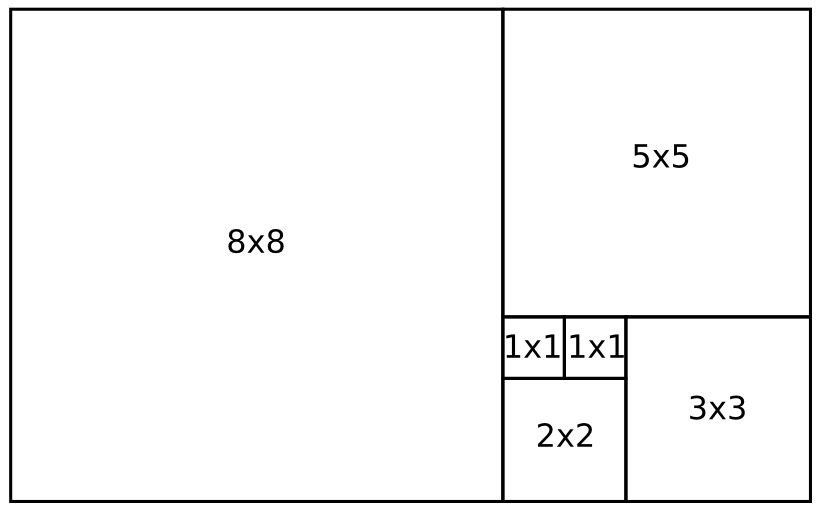
\includegraphics[scale=0.35,angle=0]{afsnit/baggrund/billeder/fib_rect}
	\end{center}
    \caption[Rektangel opbygget efter Fibonaccis talrække]{Rektangel
    opbygget efter Fibonaccis talrække. Man kan blive ved med at sætte
    $F(n)$ x $F(n)$-rektangler på denne figur og derved tilnærme sig et
    ægte gyldent rektangel jvf. tabel \ref{fibonacci_sequence}.}
	\label{fibonacci_rektangel}
\end{figure}
Vi kan nu tegne kvarte cirkler i figur \ref{fibonacci_rektangel}, med
radius $F(n)$, og derved approksimere en gylden spiral, som vist i figur
\ref{fibonacci_spiral}. Hvor tæt vi kommer på en egentlig gylden spiral
afhænger af, hvor mange rektangler vi har brugt til at tegne spiralen
efter. Et højere antal rektangler giver en spiral, som er tættere på en
egentlig gylden spiral. Formelt kan det direkte udledes af tabel
\ref{fibonacci_sequence}, hvor tæt en approksimation vi har på en gylden
spiral.
\begin{figure}[h!]
	\begin{center}
		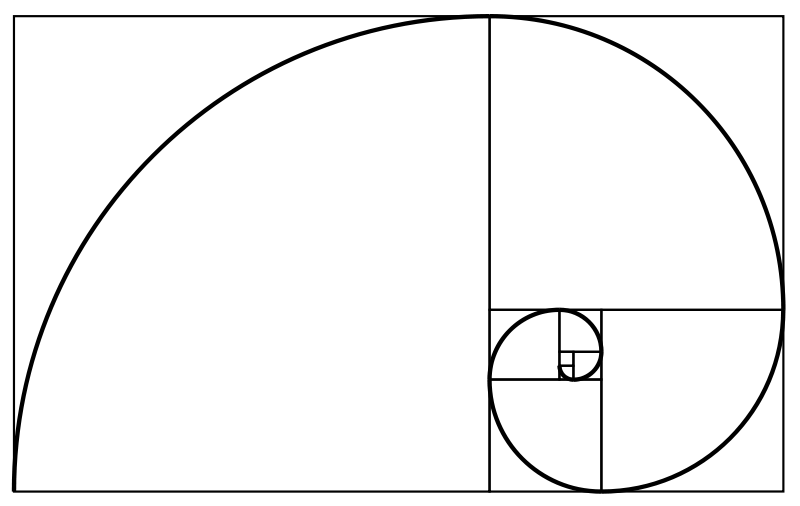
\includegraphics[scale=0.35,angle=0]{afsnit/baggrund/billeder/Fibonacci_spiral}
	\end{center}
	\caption[En fibonaccispiral]{En fibonaccispiral - \emph{Kilde: Wikipedia}}
	\label{fibonacci_spiral}
\end{figure}
Hvis man regner den korrekte faktor $c$ ud og tegner en ægte gylden
spiral i et gyldent rektangel vil man se at spiralen faktisk går
\emph{uden for} rektanglet\cite{Sharp2002}. Ovenstående approksimation,
med radius $F(n)$, vil aldrig gå ud over rektanglet, og det bliver derved
klart, at fibonaccispiralen i sandhed blot er en approksimation.

For en fuld gennemgang af spiraler, specielt med henblik på det gyldne
snit, se \cite{Sharp2002}. Vi vil nu kaste et hurtigt blik på
problematikken ved at afgøre hvad der er interessant i et billede og se
på hvordan computeren kan bruges i denne sammenhæng.

}
% vim: set tw=72 spell spelllang=da:


\section{Computeren som betragter\label{section_computer_betragter}}
{
Giver man tre forskellige mennesker den opgave at afgøre hvad der er det
interessante i et givet maleri, kan man meget vel få tre forskellige
svar. Mere kompliceret bliver det når man spørger ind til \emph{hvordan}
de er kommet frem til deres svar. Én begrunder måske sit valg med en
viden om netop det givne maleri, en anden med viden om maleriets
kunstner eller periode, mens en tredie begrunder det med æstetiske
virkemidler eller subjektive holdninger. Her er alle muligheder åbne for
at lave fejl, da man som regel ikke har kunstneren til rådighed til at
give det rigtige svar, hvis han da overhovedet selv kender det.
Maleriets motiv kan lede én på sporet af hvad der er interessant, men
dette kræver måske en viden om motivets bagvedliggende historie.
Mennesket tager altså en lang række overvejelser og baggrundsviden i
betragtning når ovenstående opgave skal løses.

Det interessante i et billede afhænger af den enkelte opgave.  Hvis vi
forestiller os en læge der kigger på et røntgenbillede af en patient som
har brækket armen, er det indlysende hvad lægen betragter som det
interessante i billedet, nemlig der hvor bruddet sidder. Når vi har med
tilfældige malerier at gøre, så står vi dog stadig tilbage med
spørgsmålet: \emph{``Hvad er egentlig \emph{interessant} i et maleri?''}
Vi lader dette spørgsmål stå åbent for at se på hvordan computeren
betragter et maleri.

\begin{figure}[h]
    \centering
    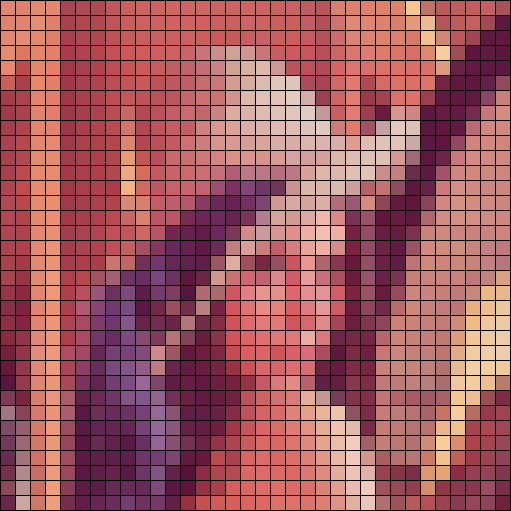
\includegraphics[scale=0.3]{afsnit/baggrund/billeder/pixel_lena}
    \caption[]{Pixels i et billede}
    \label{pixel_lena}
\end{figure}

Billedet i figur \ref{pixel_lena} er blevet delt op i nogle små felter
kaldet pixels. Hver pixel har en farve. Computeren opfatter et billede
netop som pixels. Computeren ser endvidere disse pixels \emph{én ad
gangen}. Det svarer altså til at den enkelte farve til en pixel bliver
læst op for en person der ikke kan se selve billedet. For at køre
eksemplet helt ud, så har vi at en person får følgende at vide:
\begin{quote}
    \emph{``Pixel med koordinater $(0, 0)$ er gul. Pixel med
    koordinater $(1, 0)$ er orange''} etc.
\end{quote}
Dette giver ingen egentlig information om \emph{hvad} billedet
forestiller. Computeren kan ikke se billedet i sin helhed og har som
udgangspunkt ikke nogen baggrundsviden at basere en vurdering på. Det
eneste computeren kan gøre er at gå billedet igennem pixel for pixel og
sammenligne dem.

Vi ønsker at bruge computeren til at afgøre om der ligger noget
interessant i billedet omkring det gyldne snit. Vi vil derfor nu kaste
et blik på den forskning der allerede er blevet gjort på dette område.

}

% vim: set tw=72 spell spelllang=da:


\section{Eksisterende forskning\label{section_forskning}}
{
Som allerede nævnt, kendte de gamle grækere til tallet $\varphi$, som
Euklid kaldte for \emph{the division in extreme and mean ratios},
forkortet DEMR. Luca Pacioli udgiver i 1509 bogen \emph{De divina
proportione}, som beskriver samme fænomen omtalt som ``den guddommelige
propertion''. Udtrykket ``det gyldne snit'' kan spores tilbage til
tyskeren Martin Ohm (1792 -- 1872), der første gang betegner Euklids DEMR
som \emph{der Goldener Schnitt} i sin bog \emph{Die reine
Elementar-Mathematik}, fra 1835\cite{Markowsky1992}. Det gyldne snit er
nu blevet den foretrukne betegnelse.

Nu bliver det påstået, fra flere kilder, at det gyldne snit bruges i
malerier, arkitektur og musik, da dette forhold har specielt tiltalende
æstetiske
egenskaber\cite{GoldenNumber,RatioArt,Putz1995,Stakhov2006490,Boussora2004}.
Især \cite{GoldenNumber} er særlig ivrig og finder det gyldne snit i alt
lige fra cigaretpakker til skallen fra en nautil. Netop nautilskallen
bliver meget ofte brugt som argument for, at det gyldne snit findes i
naturen i form af en gylden spiral lignende den fra figur
\ref{fibonacci_spiral}. Hvis man rent faktisk måler efter,
viser det sig, at dette ikke er tilfældet. Som argumenteret i
\cite{Sharp2002} er spiralen i nautilskallen rigtigt nok logaritmisk,
men ikke med en faktor $c$ som ville gøre den til en gylden spiral.

Det græske tempel Parthenon spiller også en central rolle i påstanden om
det gyldne snit. Billeder af templet bliver tit vist med et rektangel
tegnet over. Der florerer forskellige udgaver af disse billeder, hvor
der åbenbart ikke tages højde for, at dele af templet ikke indgår i
rektanglet eller fotografiets perspektiv. George Markowsky gør i
\cite{Markowsky1992} op med mange af disse vrangforestillinger. Påstande
om, at Keopspyramiden skulle være bygget efter det gyldne snit --- som
angivet i \cite{Stakhov2006490} --- at nogle af Leonardo da Vincis malerier
er malet efter det gyldne snit, og at det gyldne rektangel er det mest
æstetisk tiltrækkende format\cite{GoldenNumber,RatioArt}, bliver i
hans artikel afvist, da mange af disse undersøgelser lider under det, han
kalder \emph{the Pyramidology Fallacy}. Dette udtrykt henter Markowsky
fra \cite{Gardner1952_2} og beskriver de personer, der forsker i
pseudovidenskab såsom pyramidernes arkitektur. Her har forskerne ofte
mange forskellige tal at ``jonglere'' med og kan frit vælge netop dem,
der giver det ønskede resultat. En anden forfatter, Roger
Hertz-Fischler, er ligeledes optaget af den specielle værdi, det gyldne
snit er blevet tillagt. Det som Markowsky og Gardner kalder for
\emph{Pyramidology}, betegner han som \emph{golden numberism}, og han har
fulgt dette fænomens historie tilbage til en tysk mand ved navn
Adolph Zeising (1810 -- 1876)\cite{Herz-Fischler2005}. Hertz-Fischler
hævder, at stort set alle undersøgelser inden for \emph{golden numberism}
kan spores tilbage til Zeising.

Hypotesen om det gyldne rektangels æstetiske egenskaber bliver også
taget op i \cite{Boselie1984} og \cite{Plug1980}, hvor det ikke kan
konkluderes, at det gyldne rektangel skulle have nogen æstetisk
signifikans. En lignende hypotese bliver sat på prøve i
\cite{McManus1995}, hvor det undersøges, om et billedes geometriske
komposition har indflydelse på dets æstetiske effekt. I. C. McManus
kunne, gennem tre eksperimenter, ikke finde noget grundlag for, at et
billedes geometriske komposition, påvirkede testpersonernes bedømmelse.
Det siges i konklusionen:

\begin{quote}
	\emph{``Together the results of these experiments throw
	considerable doubt upon the hypothesis of the implicit detection
	of latent compositional geometry as a major component of
	aesthetic judgements, at least for relatively unsophisticated
	observers[\dots]''}
\end{quote}

Selvom ovenstående ikke eksplicit nævner det gyldne snit, har det
alligevel en klar relevans til billeder opbygget geometrisk efter det
gyldne snit.

Der ses dog et klart problem, hvilket Markowsky også nævner, idet det
ikke er defineret, hvornår et stykke kunst er konstrueret efter det
gyldne snit. Ej heller er det defineret, præcis hvordan man finder det
gyldne snit: Der findes mange billeder, hvor snittet er illustreret vha.
linjer, men størstedelen af disse har ikke de fornødne mål, og det
gyldne snit findes gerne helt arbitrære steder uden nogen som helst
identificerbar fremgangsmåde.  Én undersøgelse, omhandlende billeders
komposition, har dog lavet statistik på 565 malerier, men kun forholdet
mellem lærredets dimensioner er blevet registreret\cite{Olariu1999}.
Denne undersøgelse kunne ikke konkludere, at kunstnere foretrækker det
gyldne snit i lærredet.

Det er derfor interessant at forsøge at automatisere søgningen efter det
gyldne snit i malerier og fastsætte klare kriterier for, hvornår et
malerier indeholder objekter, som ligger i det gyldne snit.  Til denne
opgave er det oplagt at udnytte regnekraften fra computeren, for at
sikre en ensartet bedømmelse af malerierne.

\subsection{Eksisterende datalogisk forskning}
Tidligere datalogiske forskning indenfor detektion af det gyldne snit er
ikke eksisterende. Derfor bliver vi nød til at kigge på generelle teorier og algoritmer
indenfor billedbehandling, mest i retning af  analyse af interessante
regioner. Den mest relaterede forskning er et eksperiment, som
analyserer æstetik i fotografier\cite{DattaWang}.
Det væsenlige ved dette eksperiment er hvorledes billederne
bedømmes. Her arbejdes der med 56 forskellige kandidater til at definere
et billede, som er mere eller mindre æstetisk korrekt og originalt. 
Kandidaterne bliver udvalgt i forskellige kategorier, tre af
kandidaterne bliver vurderet ud fra ``The rule of Thirds'', som er 
beskrevet således.
\begin{quote}
	``The rule can be considered as a sloppy approxmination of the
	golden ratio (about 0.618)''
\end{quote}

%fyld? Meget fedt at få sagt det men jeg ved ikke om det er specielt
%vigtigt
Denne artikels kandidater dækker over noget ganske centralt i
billedbehandling nemlig detektion af
interessante regioner i billeder, problemet er at begrebet slet ikke er
entydigt defineret, men skifter betydning fra fagområde til fagområde.
Hvad vi opfatter som interessant vil blive diskuteret i \ref{section_kort_intro}

Den første er maskineindlæring, der stammer fra feltet kunstig
intelligens indenfor datalogi. I billedbehandling bliver det dog
brugt til at finde interessante regioner med stor præcision, og formålet
med brugen er blandt andet at finde ansigter, mennesker og
biler\cite{ViolaJones01,SchneidermanKanade00,Gabor}. Præcisionen på
algoritmernes detektion betyder dog en øget kompleksitet i udvikligen. 

Den anden er opdelinger af billeder efter tekstur. Ideen bag denne type
af metoder er at opdele efter
overfladetekstur\cite{218442,CarsonBelongie02,PapageorgiouPoggio}.
Der er mange forskellige algoritmer, der arbejder på så forskellige ting
som farveklatter og detektion af mønstre\cite{PalPal}.

}
% vim: set tw=72 spell spelllang=da:


\section*{Opsummering}
Den matematiske definition, giver os nogle værktøjer, til at analysere
malerier for brug af det gyldne snit.  Den eksisterende forskning, eller
mangel på samme, fortæller os, at det er en meget svær opgave, at bruge
computeren til at fortolke malerier, og at det er tvivlsomt, hvorvidt
det gyldne snit kan tillægges nogen speciel værdi.  I næste afsnit vil
vi se på, hvilke metoder vi vil bruge, for at undersøge det gyldne snit
i digitale gengivelser af malerier.

}

% vim: set tw=72 spell spelllang=da:


\chapter{Detektion af det gyldne snit}
\subsection{Opdeling af billeder}
\textsf{
Mange af de metoder, vi bruger til at udregne, det gyldne snits position
eller størrelsen af en margin, udregnes med brøker. Hvorimod et billede
opbygges af pixels. Dette gør, at vi bliver nødt til at tage
approksimationer af udregningerne. Vi vil også kommer ind på nogle af de
fejl som kan opstå i tilblivelse af maleriet}

\subsection{Inddeling af billede efter snit}
Vi vil i dette afsnit give nogle definitioner på hvordan et billedet er
bygget op, samt hvilke afrundings fejl der kan opstår ved denne
opbygning. For at få nogle faste definitioner på hvordan et billedet ser
ud samt hvad et snit er, har vi stillet de her to definitioner op.

\begin{definition}
	I et billede betegnes \textbf{højden og bredden} som hhv. $H$ og
	$B$, som illustreres i figur \ref{cut}.
\end{definition}

\begin{definition}
	Et \textbf{snit} er en lige vertikale eller horisont linje, som
	strækker sig fra kant til kant.
\end{definition}

\begin{figure}[h]
	\begin{center}
		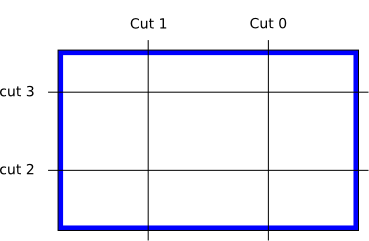
\includegraphics[scale=0.42,angle=0]{afsnit/vores_implementation/billeder/naiv_algoritme/Cut}
	\end{center}
	\caption[]{Billedets højde og bredde betegnes hvv. H og B. De 4 snit er navngivet.}
	\label{cut}
\end{figure}

End til vider har vi kun arbejder med det gyldne snit, men andre snit i
billedet kan godt optræde, derfor indføre vi en nu betegnelse
snitratio.

\begin{definition}
	En \textbf{snitratio} er en procents sats, som ganget på $B$ eller
	$H$, finde placeringen af et snit i billedet.
\end{definition}

Det vil sige at hvis en snitration er på $0.2$. Et billedet har $B$ på
4000 vil et snit befinde sig i pixel $4000*0.2 = 800$ fra højre side af
billedet, det samme antal pixel fra venstre side vil også være et snit.
Samme metode kan bruges på $H$ for at få 2 snit mere. 

\begin{definition}
	For vær snitration er der fire snit, to i det vertikale plan og to i
	det horisontale plan, som er illustreret på maleri \ref{lenasnit2},
	med røde streger. Med mindre snitration er 0.5, så er der kun 2 snit.
\end{definition}

Hvis snitratioen er $0.5$ kommer snittene til at ligge over på hinanden,
og derved vil snitratioen kun have 2 snit, de 2 snit Id, samt snitenes
plascring kan ses i figur \ref{2Cut}.

\begin{figure}[h]
	\begin{center}
		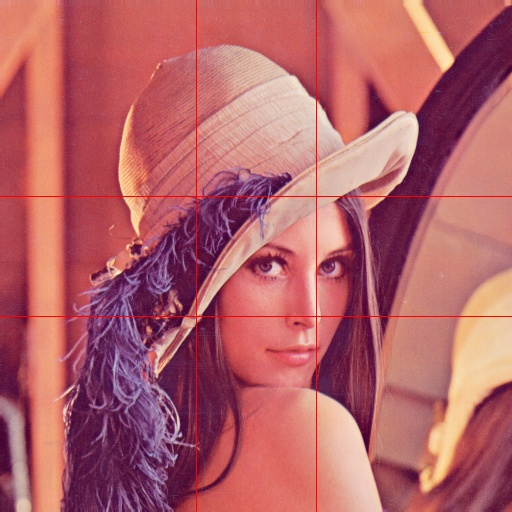
\includegraphics[scale=0.42,angle=0]{afsnit/vores_implementation/billeder/naiv_algoritme/Lenagolden}
	\end{center}
	\caption[]{Billedet som har indtegnet de fire gyldne snit}
	\label{lenasnit2}
\end{figure}

De 4 snit tildeles hvert deres Id, "snit 0,1,2 og 3" så vi kan kende
forskel på de individuelde snit, Id'erne placering kan ses i figur
\ref{cut}. Vi vil i resten af rapporten kalde snittene efter deres Id.

\begin{definition}
	Vær snit af vær snitratio, har et fast \textbf{Id}, "Snit 0,1,2 og 3", som kan ses i figur \ref{cut}, hvor vært snit er indtegnet, samt deres Id som label. 
\end{definition}

\begin{figure}[h]
	\begin{center}
		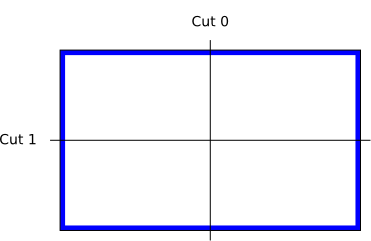
\includegraphics[scale=0.42,angle=0]{afsnit/vores_implementation/billeder/naiv_algoritme/2Cut}
	\end{center}
	\caption[]{Billedet skæres her kun af 2 snit}
	\label{2Cut}
\end{figure}

\subsection{Acceptabel afvigelse}
\begin{comment}"""
Som beskravet i afsnit \ref{mange_tal}, udregnes det gyldne snit med mange decimaler. Selv den beste kunstner har et maksimum på hvor præcis han kan male, om det er hans øjne der sætter grandsen eller størrelsen på han pensler eller om han bare ikke maler særlige præcis, så kan han aldrig malle så præcis som vi kan udregne det gyldne snit til. Derfor sætter vi en afvigelse på $0.5 \%$, som maleren vi sat en 
\end{comment}
\note{Nogle referanse}Som beskrevet i afsnit \ref{mange_tal}, udregnes
det gyldne snit med mange decimaler. En kunstner, hvor god han end er,
har ingen chance for at male så præcist at man kan sige at strøget
ligger nøjagtigt oven på snittet selv om hans intentioner er at ramme
snittet. Vi kommer derfor til at have en vis uprecis hed på de data vi
få fra billedet selv. Vi starter med at se på alle de ting, som kan
skabe en usikkerhed fra malerens side. Man kan gå ud fra at den
procentvise afvigelse ikke er særlig stor, da vi ikke har bestræbelser
på at arbejde på abstrakt malerier, dog har vi sat den procentvise
afvigelse til 0.5 \%. Det vil sige at en maler med et lærred på 100
cm, maksimalt vil male $0.5$ cm forkert.

Når maleren vælger en ramme og et lærred, har vi igen problematikken,
selv om maleren spicifikt gå efter at bygge maleriet op efter det gyldne
snit, kan snittets placering i maleriet have forskubbet sig, ved dårlige
valg at ramme eller lærred. Derfor sætter vi den afvigelse til $1\%$. Da
vi igen mener at dette er den maksimale afvigelse, der kan opstå.

Når maleren maler en region i et maleri, forekommerer der normalt en
lille kant rundt om objektet, et omrids. Dette omrids kan vores
algoritmer ikke tage højde for, og vi må derfor modregne omridset, så vi
er sikre på at vi ser på regionen og ikke dens omrids. Da et omrids ikke
er særligt stort, har vi sat denne procentsats til $0.5\%$. 

Alt i alt giver det en afvigelse på vores aktuelle udtrækning af data
fra malerierne på $2\%$ det vil sige at finder vi en region, som ligger
på pixel 200, i et billedet, der er $500$ cm bredt, befinder den sig
faktisk i intervallet [190,210]. Måden hvorpå vi tager højde for den
forskel, er ved hjælp af marginer, som nævnt i afsnit
\ref{section_naiv}.


\subsection{Heltal i det gyldne snit}
Nå vi udregner hvor et snit for et billedet med $H = 4000$,
approksimerer vi antal pixels ved at afrunde resultatet $2472.13595
\approx 2472$, se udregning \ref{afrundning}. Det betyder at vi mister
0.13595 pixels i præction, hvilket svarer til en misvisning af punktet
på 0.00339875 $\%$ i forholdt til $B$ på billedet. Se udregning
\ref{afrundning2}.

\begin{equation}
	4000 \cdot \varPhi = 4000(\sqrt{5}-1)/2 = 2472.13595 \approx 2472 \label{afrundning}
\end{equation}

\begin{equation}
	0.13595/4000 \cdot 100 = 0.00339875 \label{afrundning2}
\end{equation}

Det er en meget lille del af selve billedet og skulle ikke give nogle
misvisninger i forhold til udregningen. For at gøre det lidt mere
generelt, sætter vi trunkeringsfejlen til $0.5$, da det er den maksimale
afrundingsfacktor som kan forekomme. Hvis billedet har en størrelse på
500 pixels, hvilket er det mindste billedet vi har, giver dette en fejlmargin
på $0.1 \%$. Dette tal bliver adderet til fejlsatsen ovenfor, og giver
en samlet afvigelse på $2.1\%$.



\subsection{Heltal ved udregning af Margin}
Når vi har 2 forskellige snitratioer, f.eks. $\varPhi$ og $\frac{2}{3}$,
som ligger meget tæt på hinanden, og vi gerne vil sammenligne hvilken
regioner der ligger i snitratioernens snit, er det vigtigt at margin for
vært af de 2 snitratioers snit ikke krydser hinanden. 

Hvis margin krydser. Vil det indebære, at den samme region bliver fundet
af begge snit. Dette vil give et skævt billedet af forskellen på de to.
Derfor må vi sørge for at marginerne ikke krydser. Hvis $x$ betegner
antal pixels i $B$ eller $H$, og vi vil se på, hvor mange pixels, der er
mellem snitratio $\frac{2}{3}$ og $\varPhi$, multiplicerer vi $x$ med de
to snitratioen for at finde deres placering. Derefter subtraheres vi et
af de snit som befinder sig tetest på hinanden i vær snitratio med
hinanden.


\begin{eqnarray}
	\frac{x2}{3} - \frac{x2}{\sqrt{5}+1} & = & x(\frac{2}{3} - \frac{2}{\sqrt{5} + 1}) \nonumber \\
	& = & x(0.666667-0.618034) \\ \nonumber
	& = & x(0.048633)
\end{eqnarray}

Vi har nu fundet antal pixel mellem de to snit. Vi vil gerne undgå at
de to marginer krydser hinanden, så vi dividere antal pixel mellem de to snit med to og afrunder værdien.

\begin{equation}
	\left\lfloor \frac{0.048633x}{2}\right\rfloor = \left\lfloor0.024316x \right\rfloor
	\label{marginstoerlse}
\end{equation}

Den minimale procentvise størrelse, margin må have, når vi
sammenligner det gyldne snit og $\frac{2}{3}$, er altså $2.4316$ Det
betyder også, at vi ikke må sammenligne snit som ligger særlig meget
tætter på hinanden, da $2.1\%$ er den minimale procent margin som vi må
have. For at vise, hvor stor marginen egentlige kan være, bruger vi formel \ref{marginstoerlse} på to billeder, et, som svarer til vores mindste billede, på
500 pixels, og et, som svarer til vores største billede, på 4000 pixels. Ved
500 pixels bliver resultatet.

\begin{definition}
	Margins størrelse i et snit, må ikke overstige $2.4316 \%$, af det respektive maleri $B$ eller $H$.
	\label{margin_max}
\end{definition}

\begin{definition}
	Margins størrelse i et snit, må ikke kommer under $2.1 \%$, af det respektice maleri $B$ eller $H$.
	\label{margin_min}
\end{definition}

\note{Er det denne måde det skal stilles op?}
\begin{equation}
	 \lfloor 500(0.024316)\rfloor = 12
\end{equation}

Det er en fin margin, da vores fejl på udregningerne ligger på 2.1 \%,
som svarer til $\lceil 500*0.021 \rceil = 11$ pixels. Der er 1 pixel fra vores
margin.

Ved 4000 pixels giver det.

\begin{equation}
	 \left\lfloor 4000(0.024316)\right\rfloor = 97
\end{equation}

Som også er god nok, da $4000*0.021 = 84$ pixels.
% vim: set tw=72 spell spelllang=da:

\subsection{Database}
{
Når vi har trukket regioner ud af billedet og vurderet dem efter
ovenstående simple algoritme kan vi stå tilbage med et egentligt
resultat. Vi ønsker at gemme dette resultat i en database så vi på et
senere tidspunkt kan bruge det i en samlet analyse af resultaterne.
Vi så i afsnit \ref{section_opbv_billeder} på et databaseskema til
opbevaring af maleriers metadata. Vi bygger nu videre på dette skema så
vi kan tilknytte resultater fra en analyse til de enkelte malerier. Det
fulde databaseskema ses nedenfor.

\begin{table}[!h]
    \centering
    \begin{tabular}{|l||c|c|c|c|c|c|}
        \hline
        \bf{artist} \hspace{0.5cm} & \underline{artistId} & name & born & died & school & timeline \\\hline
    \end{tabular}
    \caption{Databasetabel for kunstner}
    \label{artistTable}
\end{table}

\begin{table}[!h]
    \centering
    \begin{tabular}{|l||c|c|c|c|c|c}
        \hline
        \bf{painting} \hspace{0.5cm} & \underline{paintingId} & artistId & title & date & paint & $\cdots$ \\\hline
    \end{tabular}\\ \vspace{0.2cm}\hspace{1.2cm}
    \begin{tabular}{c|c|c|c|c|c|c}
        \hline
        $\cdots$ & material & location & url & form & type & $\cdots$ \\\hline
    \end{tabular}\\ \vspace{0.2cm}\hspace{1.4cm}
    \begin{tabular}{c|c|c|c|c|c|}
        \hline
        $\cdots$ & realHeight & realWidth & height & width & filepath \\\hline
    \end{tabular}
    \caption{Databasetabel for malerier}
    \label{paintingTable}
\end{table}

\begin{table}[!h]
    \centering
    \begin{tabular}{|l||c|c|c|c|c|c|c|}
        \hline
        \bf{run} \hspace{0.5cm} & \underline{runId} & trsh1 & trsh2 & lo & up & marginPercentage & method \\\hline
    \end{tabular}
    \caption{Databasetabel for en kørsel}
    \label{runTable}
\end{table}

\begin{table}[!h]
    \centering
    \begin{tabular}{|l||c|c|c|c|c|c|}
        \hline
        \bf{result} \hspace{0.5cm} & \underline{resultId} & runId & paintingId & cutRatio & cutNo & numberOfRegions \\\hline
    \end{tabular}
    \caption{Databasetabel for resultater}
    \label{resultTable}
\end{table}

\begin{table}[!h]
    \centering
    \begin{tabular}{|l||c|c|c|c|c|c|c|}
        \hline
        \bf{region} \hspace{0.5cm} & \underline{regionId} & resultId & x & y & height & width & area \\\hline
    \end{tabular}
    \caption{Databasetabel for regioner}
    \label{regionTable}
\end{table}

Tabellerne \ref{artistTable} og \ref{paintingTable} er de samme som vist
i afsnit \ref{section_opbv_billeder}, men er taget med her blot for at
vise databaseskemaet i sin helhed. Det øvrige databaseskema lægger vægt
på at minimere redundans og mulighed for at genskabe kørte analyser.
Sidstnævnte er vigtig osv\dots

}
% vim: set tw=72 spell spelllang=da:



\chapter{Afprøvning}
{
I dette Kapitel vil vi afprøve vores 2 metoder på XX(hvormange) billeder og se hvordan de virker. Udover det vil vi finde tærskelværdier til kandetection, floodfill og margin, ud fra observationer gjort under afprøvning. Vi vil også afprøve den generalle region detektor og kommer ind på dens fordele og ulemper. 
\section{Tærskelværdier}
I vores program er der 3 forskellige tærskelværdier som påvirker hvordan
metoden analysere billedet. Marginens brede, afvigelsen af farven i
floodfill og afvigelsen i farven i kandtdetectionen. Alle 3 tærskelværdier er
blevet introduceret i deres respektive afsnit, men ingen konkrate tal
er opgivet. I dette afsnit vil vi opgive de tal, samt en forklaring på
hvorfor vi har valt lige de tal.

\subsection{Marginens brede}
Vi regner marginens brede, $MB$ ud fra en procent af billedets brede og
højde. I afsnittet \ref{opdeling_af_billeder.tex} kom vi frem til en
usikkerhed på $2.1 \%$. Så vores $MB$ skal mindst
være på $2.1 \%$. Ud over det er den minimale forskel på 2 snit vi foretager os,
forskellen mellem det gyldne snit og $\frac{2}{3}$, som vi udregnet i
sektion \ref{opdeling_af_billeder.tex} til maksimalt at have en $MB$ på
$2.43$, for at margin ikke krydser. Så $MB \in [2.1, 2.43]$. Vi har valt
at sætte $MB = 2.4$, da vi derved kan tage højde for uforresette
usikkerhed. XXX(er det en dog nok forklaring).

\subsection{Afvigelsen af farver i kandtdetection}
Det vi bruger kandtdetection til, er af finde en kanter rundt om de
regioner som vi mener er interessante, og undgå de kanter som ligger
inde i regioner. Begge de 2 mål kan ikke altid opfyldes, men vi kan
komme så tæt på et krompromi mellem en perfekt kant rund om region og
ingen kanter inde i region som mulige. Dette gøres ved at ændre 2
tærskelværdier i kantdetectionen ud for observationer som vi har taget
på billederne i forvejen. Vi har valt at dele billederne som vi
observere op i 9 kategorier, som kan ses i tabel
\ref{thressholdsTabelKant}, Kategorier er en grove opdeling af
billederne efter detaljer og farve intensitet, som bruges til at give en
bedre indblik på billedets opbygning. 

\subsubsection{Sammenligninger}
Vi har set på XX(hvor mange) antal malerier og har fundet de
tærskelværdier som vi mener passer bæst på billedet. Vi vil illustrerer
den fremgange måden vi har brugt til at finde tærskelværdierne på, på
maleriet \ref{kDetalier}. Maleriet er malet med mange farver og med
masser af detaljer. Vi ser først på tærskelværdierne
$[0,0],[100,100]......[900,900],[1000,1000]$ se figur \ref{allesammen1}
og \ref{allesammen2}, og finde det interval hvor malerriet ikke har
mistet nogle af kanterne rundt om regionerne i nu, men vil det, i næste
interval. I illustration vurdere vi det til billedet \ref{300-300}, da
billedet \ref{400-400} har mistet for mange af de kanter, som vi gerne
vil beholde. Så tærskelværdien som vi gerne vil finde frem til, befinder
sig fra $[300,300]$ og frem. Ved at sætte den anden tærskelværdig op
lidt af gangen kan vi igen få en række billeder at vælge imellem, for at
få det beste resultat, se sammenligningen i figur \ref{allesammen3}. som
man kan se begynder det er være svær at skelne figurene i \ref{300-850}
og der er lidt for mange kanter i \ref{300-700}, så vi har valt at bruge
tærskeværdigerne $[300,750]$ for dette billedet. Man kunne god gå længer
ned og se om tærskeværdig $[300,745]$ passet bedre, men vi har valt at
holde . Det maleri vi lige har brugt er ikke særlige repræsentativ for
helle vores maleri database, så vi har taget en række billeder og brugt
samme metode på dem og kommer frem til en middel tærskelværdi, jeg viser
her en lille udsnit af dem, se figur \ref{en}, \ref{to} og \ref{tre}.

\begin{figure}[p]
    \centering
    \subfloat[100,100]{
        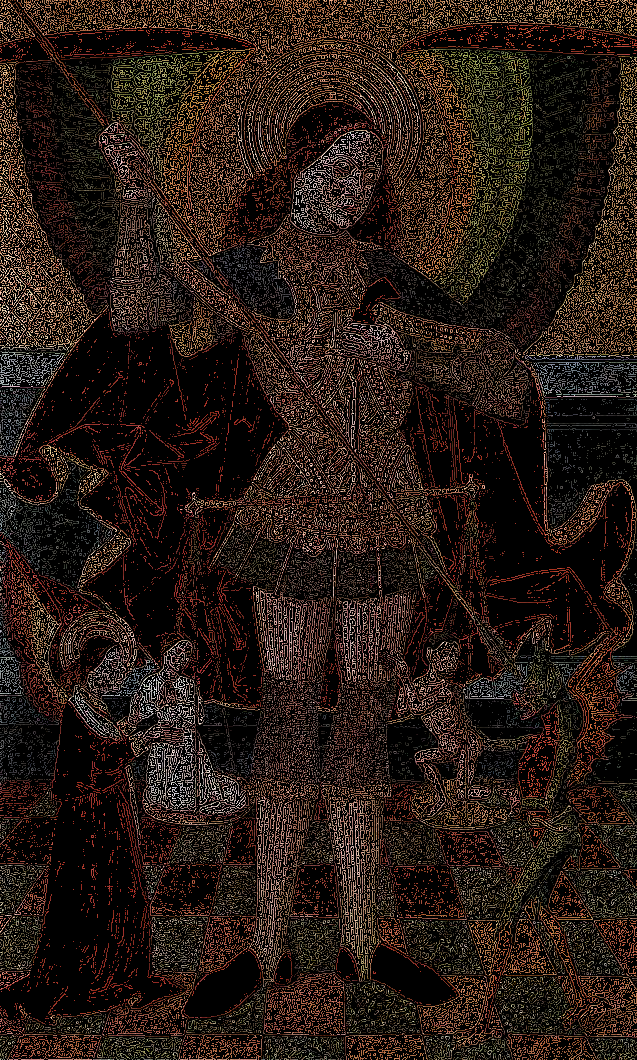
\includegraphics[angle=0,width=0.45\textwidth]{afsnit/afprovning/billeder/thressholds/krafitige_farver/krafite_detalier/1_iteration/100-100.png}
        \label{100-100}}\hspace{1em}
    \subfloat[200,200]{
        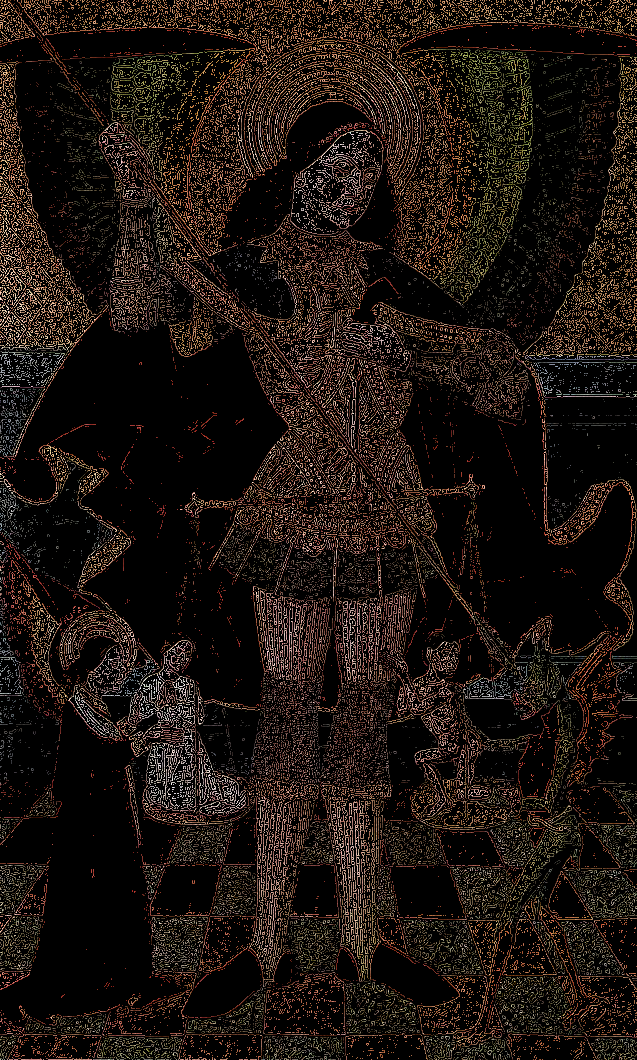
\includegraphics[angle=0,width=0.45\textwidth]{afsnit/afprovning/billeder/thressholds/krafitige_farver/krafite_detalier/1_iteration/200-200.png}
        \label{200-200}}\\
    \subfloat[300,300]{
        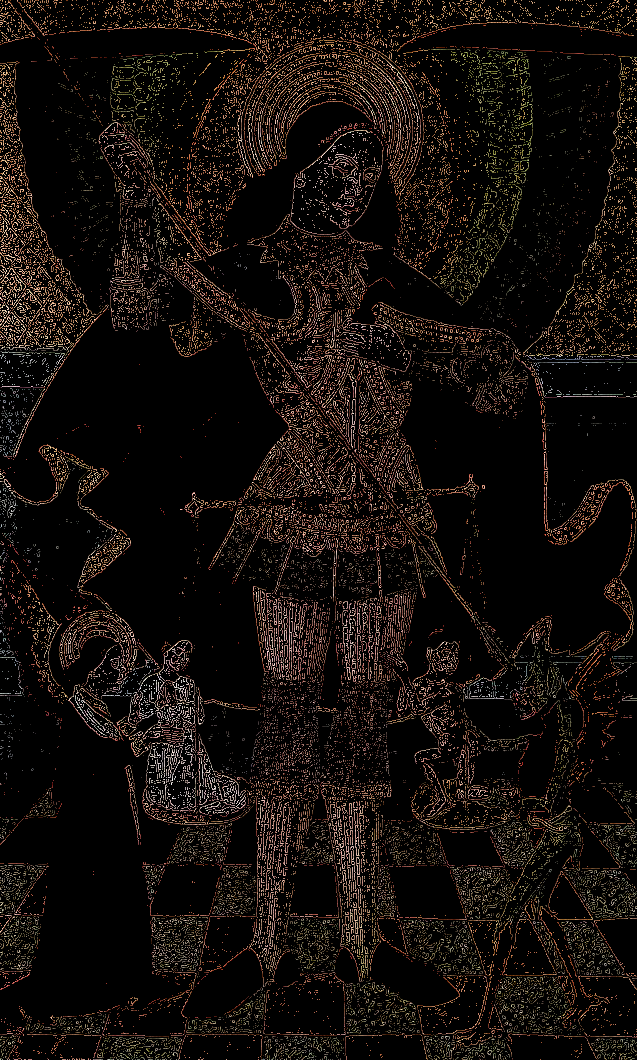
\includegraphics[angle=0,width=0.45\textwidth]{afsnit/afprovning/billeder/thressholds/krafitige_farver/krafite_detalier/1_iteration/300-300.png}
        \label{300-300}}\hspace{1em}
    \subfloat[400,400]{
        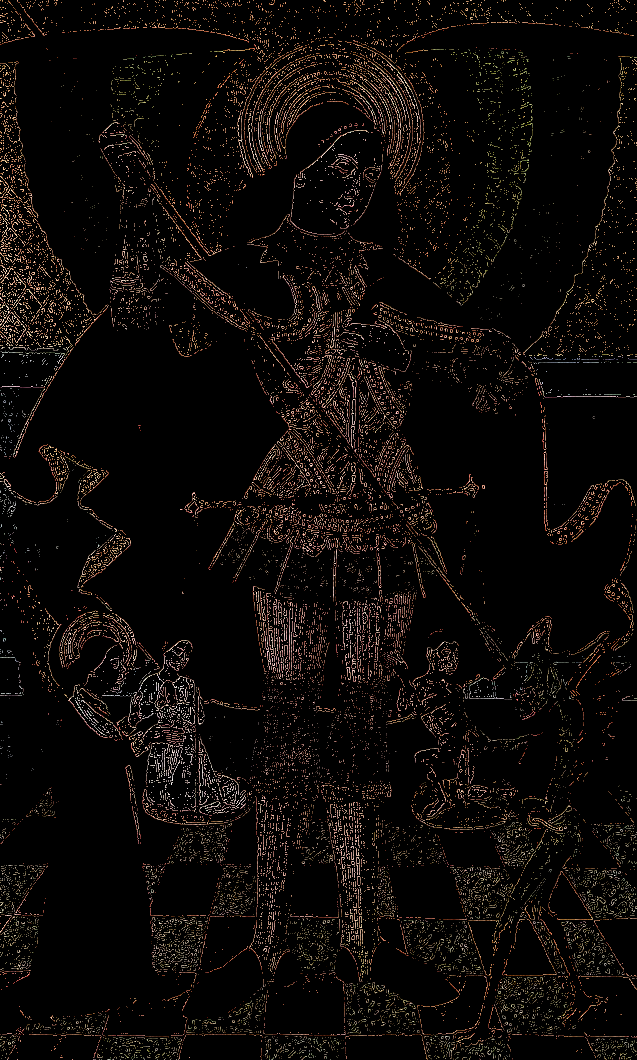
\includegraphics[angle=0,width=0.45\textwidth]{afsnit/afprovning/billeder/thressholds/krafitige_farver/krafite_detalier/1_iteration/400-400.png}
        \label{400-400}}
    \label{allesammen1}
    \caption{Hvad er et her?}
\end{figure}

\clearpage

\begin{figure}[!h]
	\centering
	\subfloat[500,500]{
        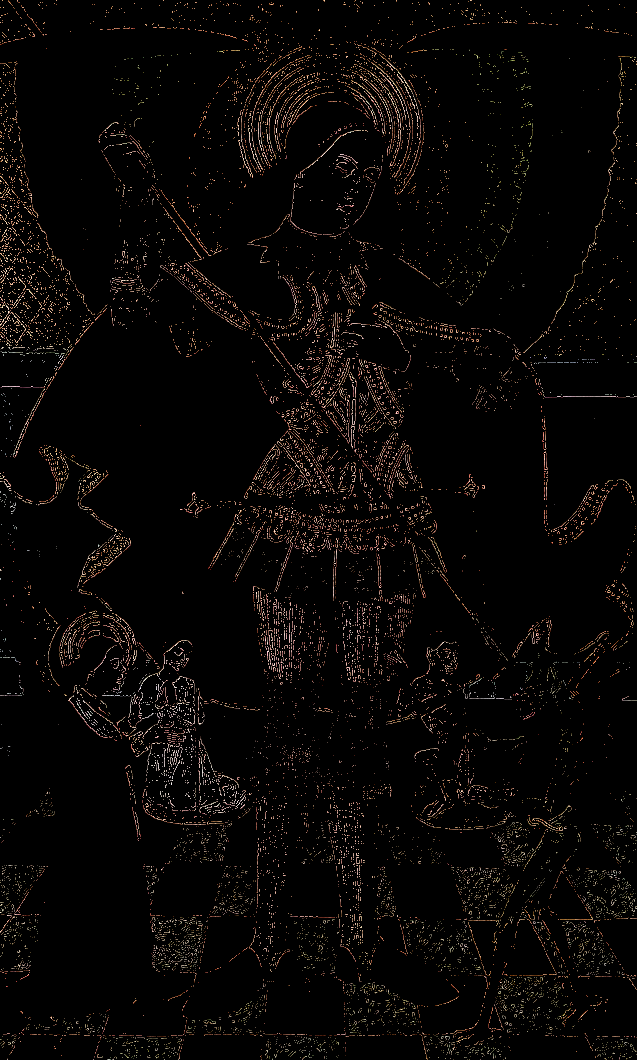
\includegraphics[angle=0,width=0.45\textwidth]{afsnit/afprovning/billeder/thressholds/krafitige_farver/krafite_detalier/1_iteration/500-500.png}
        \label{500-500}}\hspace{1em}
    \subfloat[600,600]{
        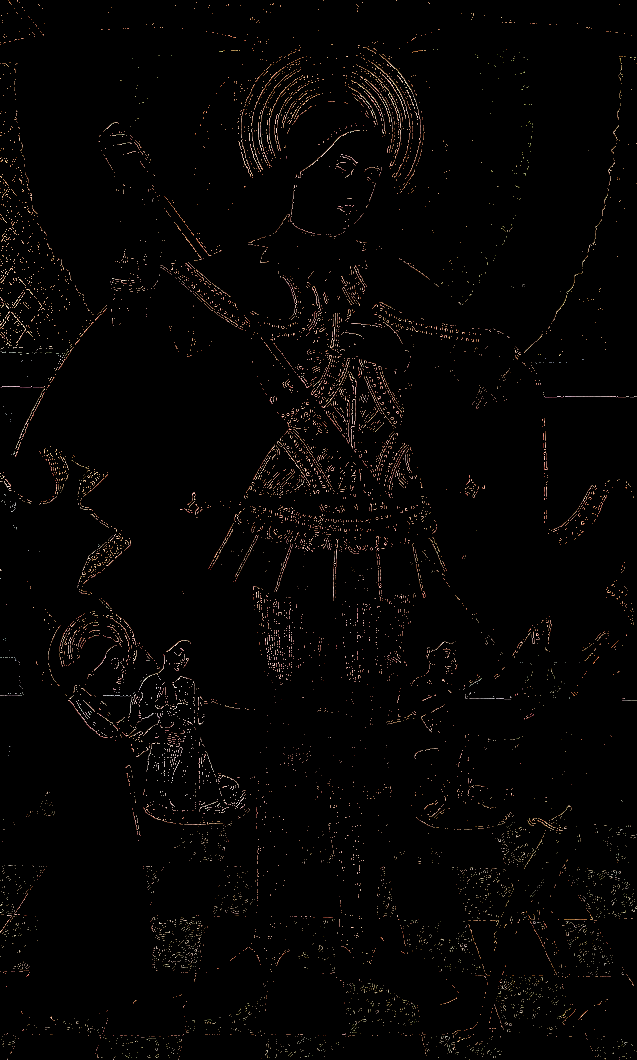
\includegraphics[angle=0,width=0.45\textwidth]{afsnit/afprovning/billeder/thressholds/krafitige_farver/krafite_detalier/1_iteration/600-600.png}
        \label{600-600}}\\
    \subfloat[700,700]{
        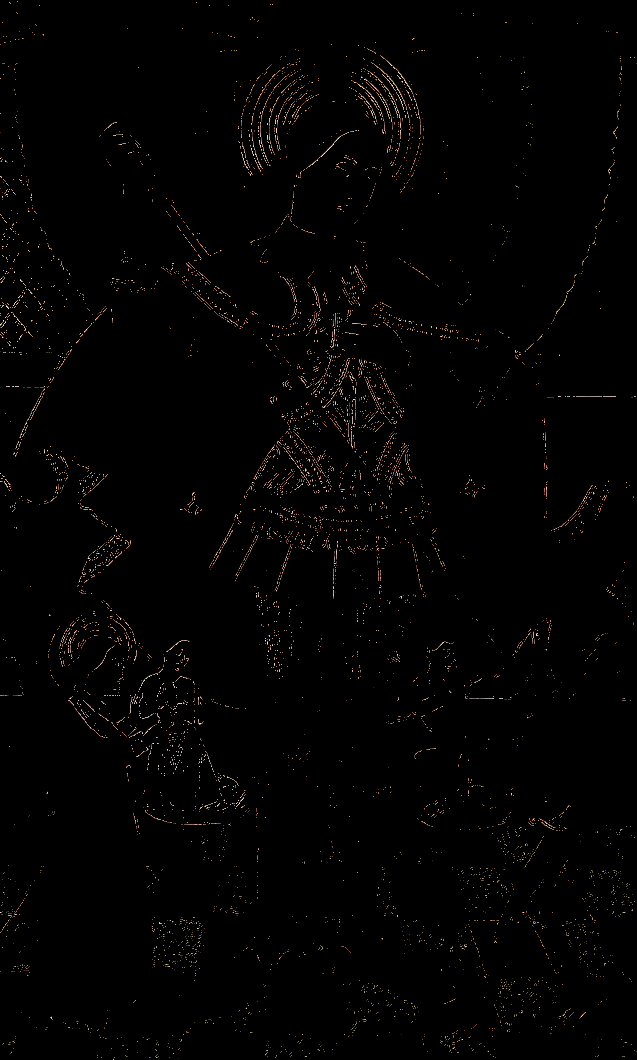
\includegraphics[angle=0,width=0.45\textwidth]{afsnit/afprovning/billeder/thressholds/krafitige_farver/krafite_detalier/1_iteration/700-700.png}
        \label{700-700}}\hspace{1em}
    \subfloat[Original]{
        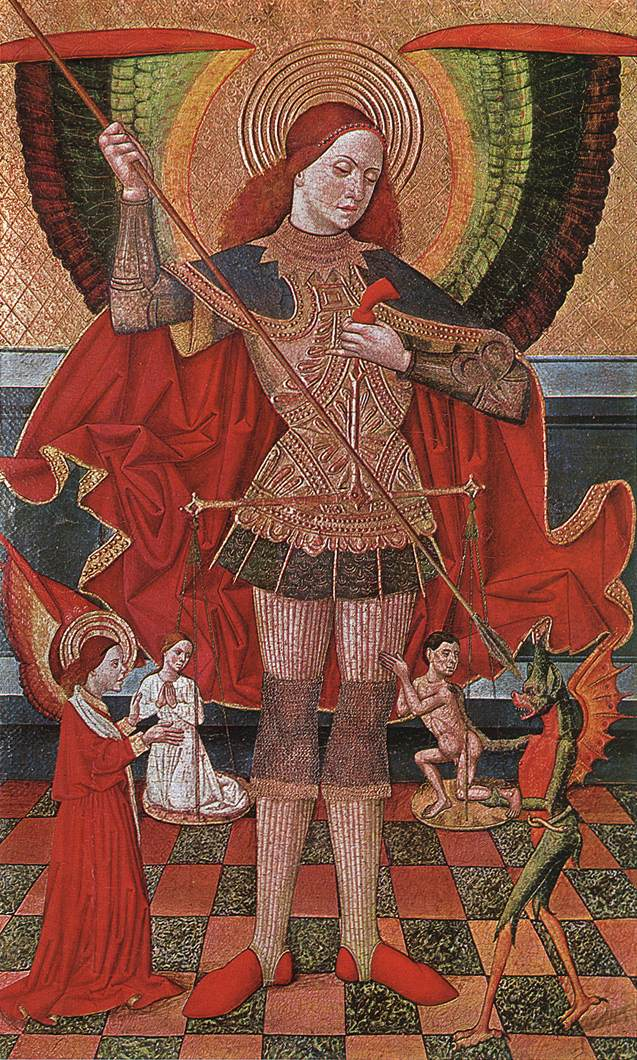
\includegraphics[angle=0,width=0.45\textwidth]{afsnit/afprovning/billeder/thressholds/krafitige_farver/krafite_detalier/kDetalier.jpg}
        \label{kDetalier}}
    \caption[]{Edgedetection på maleriet \ref{kDetalier} som har mange detaliger og kraftige farver, med tærskelværdierne fra 100-100 til 700-700}
     \label{allesammen2}
\end{figure}

\begin{figure}[!h]
    \centering
    \subfloat[300,700]{
        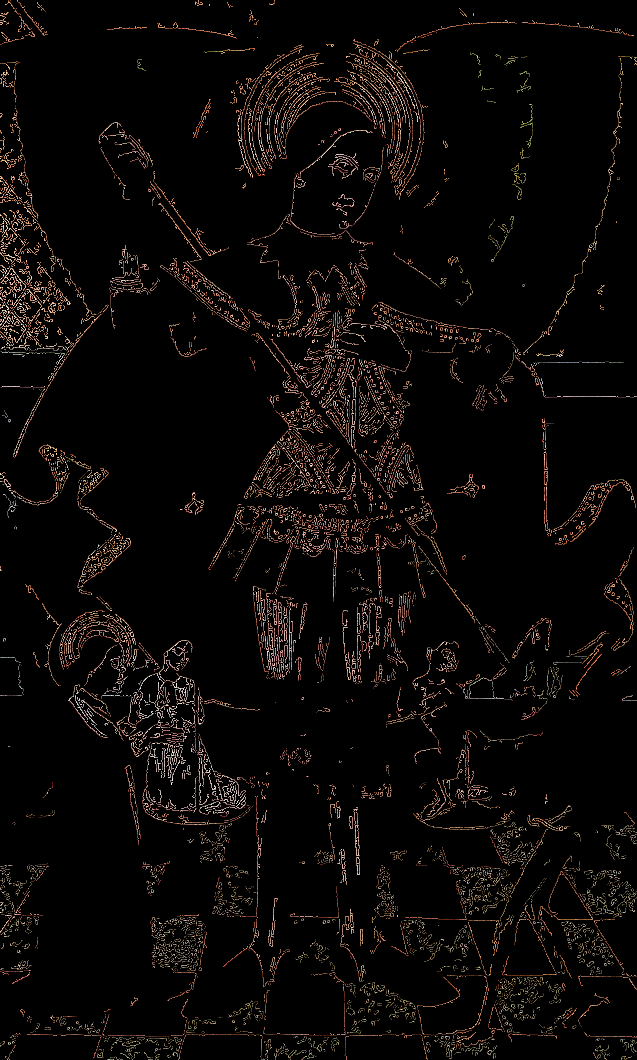
\includegraphics[angle=0,width=0.45\textwidth]{afsnit/afprovning/billeder/thressholds/krafitige_farver/krafite_detalier/2_iteration/300-700.png}
        \label{300-700}}\hspace{1em}
    \subfloat[300,750]{
        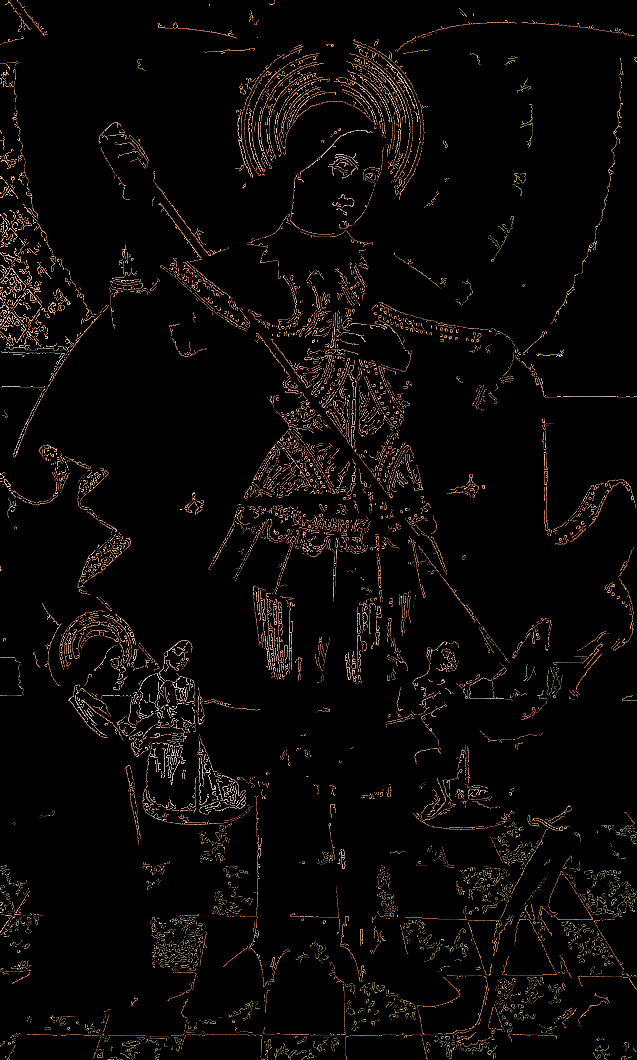
\includegraphics[angle=0,width=0.45\textwidth]{afsnit/afprovning/billeder/thressholds/krafitige_farver/krafite_detalier/2_iteration/300-750.png}
        \label{300-750}}\\
    \subfloat[300,800]{
        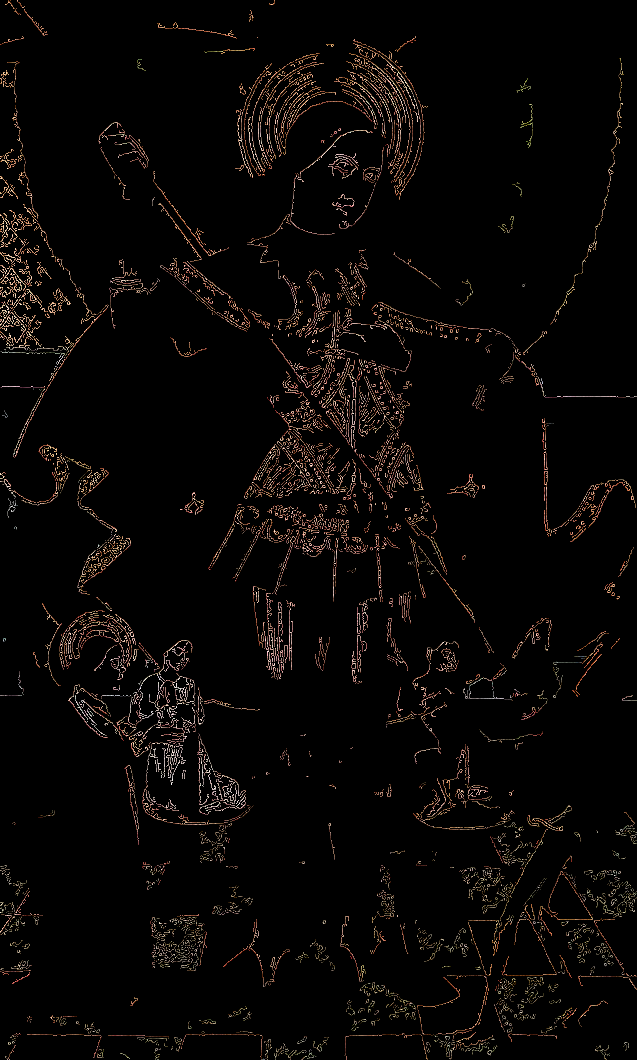
\includegraphics[angle=0,width=0.45\textwidth]{afsnit/afprovning/billeder/thressholds/krafitige_farver/krafite_detalier/2_iteration/300-800.png}
        \label{300-800}}\hspace{1em}
    \subfloat[300,850]{
        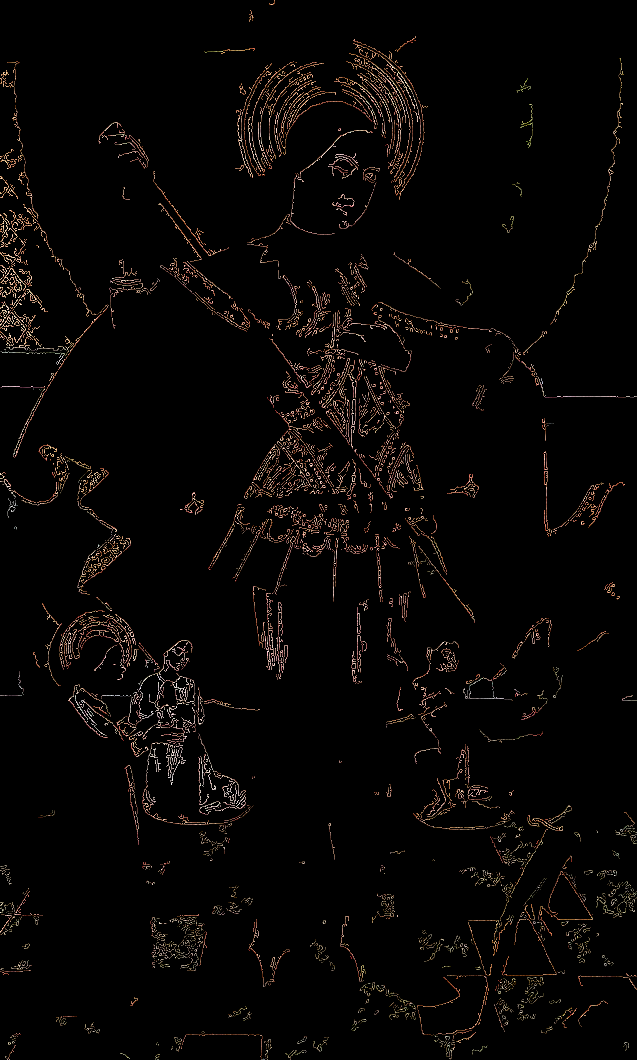
\includegraphics[angle=0,width=0.45\textwidth]{afsnit/afprovning/billeder/thressholds/krafitige_farver/krafite_detalier/2_iteration/300-850.png}
        \label{300-850}}
        \caption[]{Edgedetection hvor de 4 billeder som er intrasante taget med}
     \label{allesammen3}
\end{figure}
 
\begin{figure}[!h]
    \centering
    \subfloat[100,250]{
        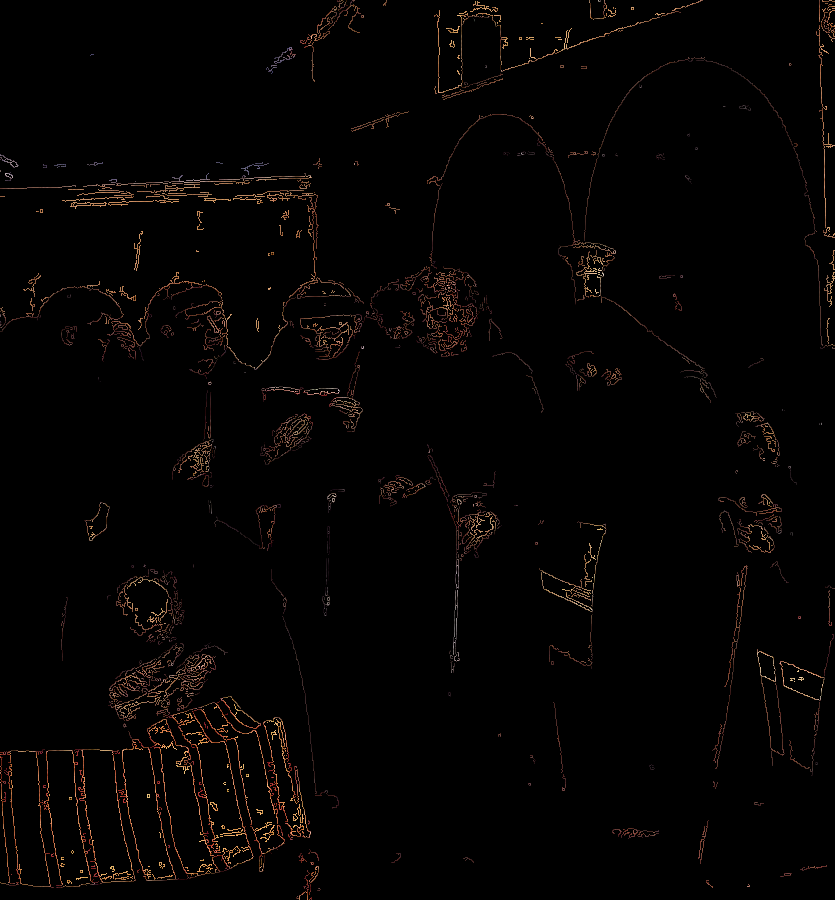
\includegraphics[angle=0,width=0.45\textwidth]{afsnit/afprovning/billeder/thressholds/svage_farver/svage_detalier/2_iteration/100-250.png}
        \label{100-250}}\hspace{1em}
    \subfloat[Orginal]{
        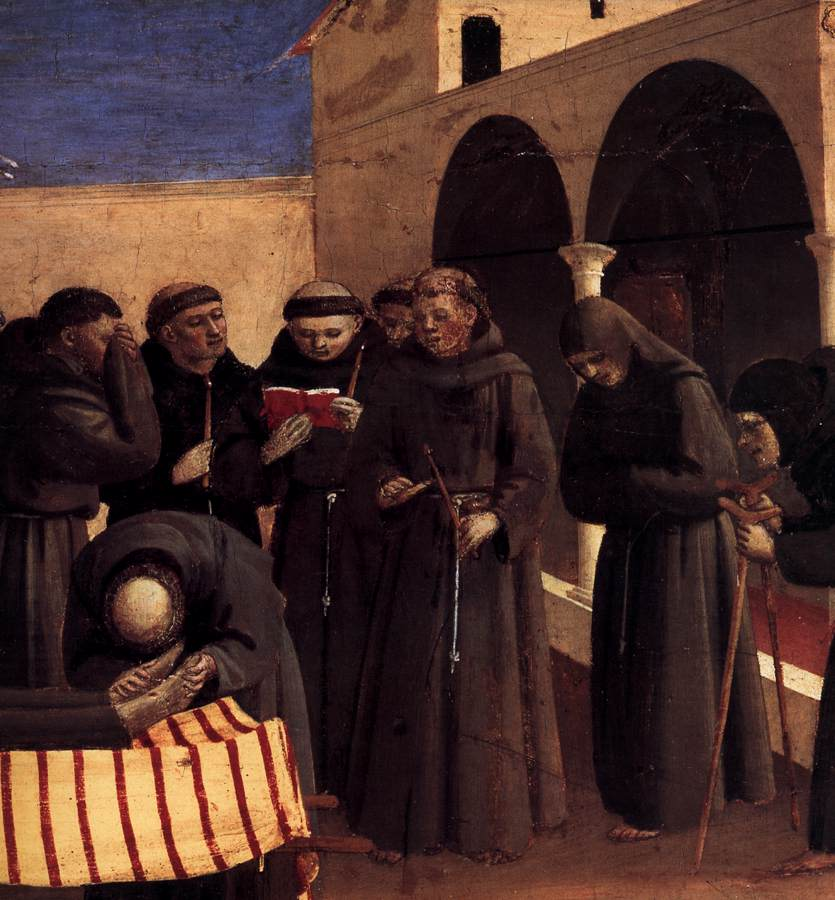
\includegraphics[angle=0,width=0.45\textwidth]{afsnit/afprovning/billeder/thressholds/svage_farver/svage_detalier/sDetalier.jpg}
        \label{Orginal1}}
        \caption[]{Edgedetection på et billedet med svage farver og få detalier, hvor tærskenværdigern [100,250] er den beste}
     \label{en}
\end{figure}

\begin{figure}[!h]
    \centering
    \subfloat[100,240]{
        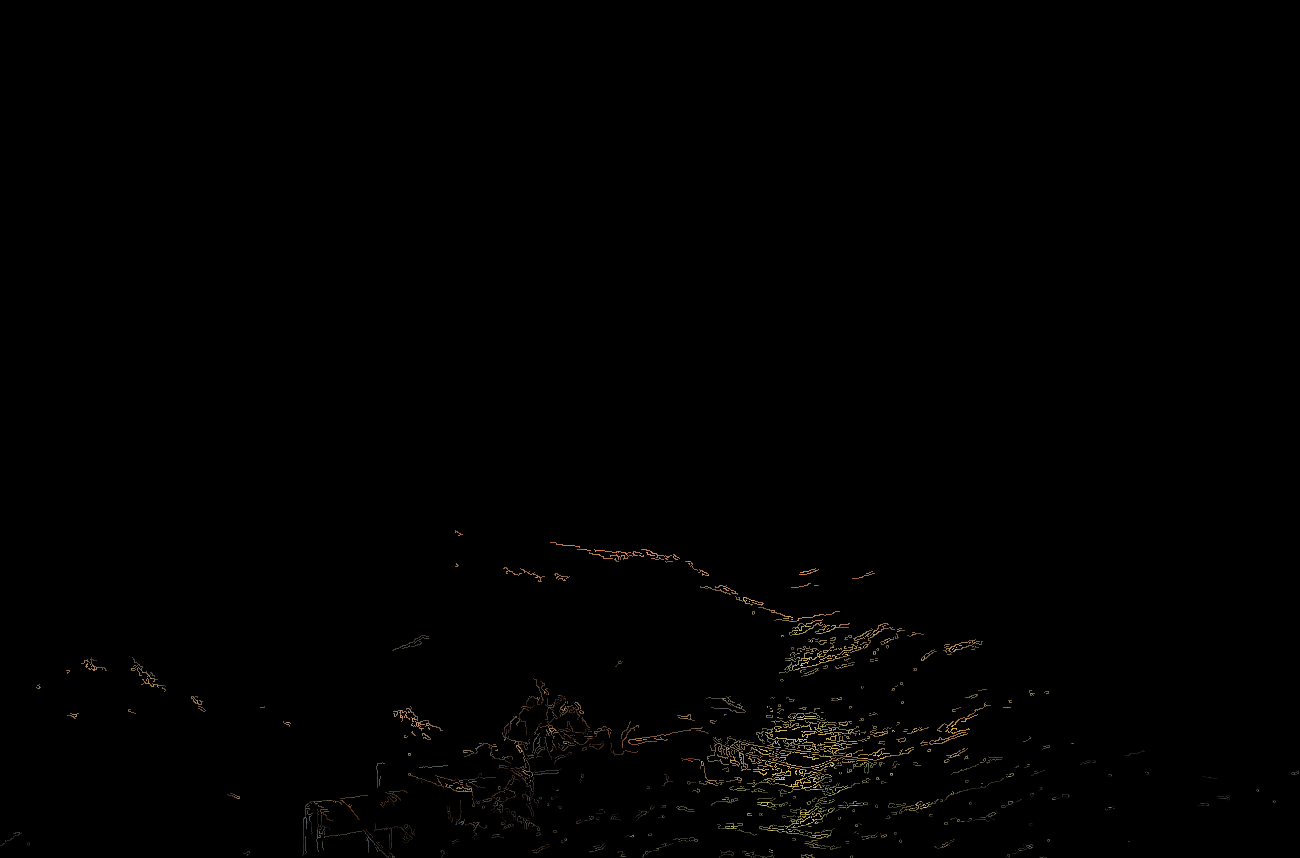
\includegraphics[angle=0,width=0.85\textwidth]{afsnit/afprovning/billeder/thressholds/medium_farver/svage_detalier/2_iteration/100-240.png}
        \label{100-240}}\\
    \subfloat[Orginal]{
        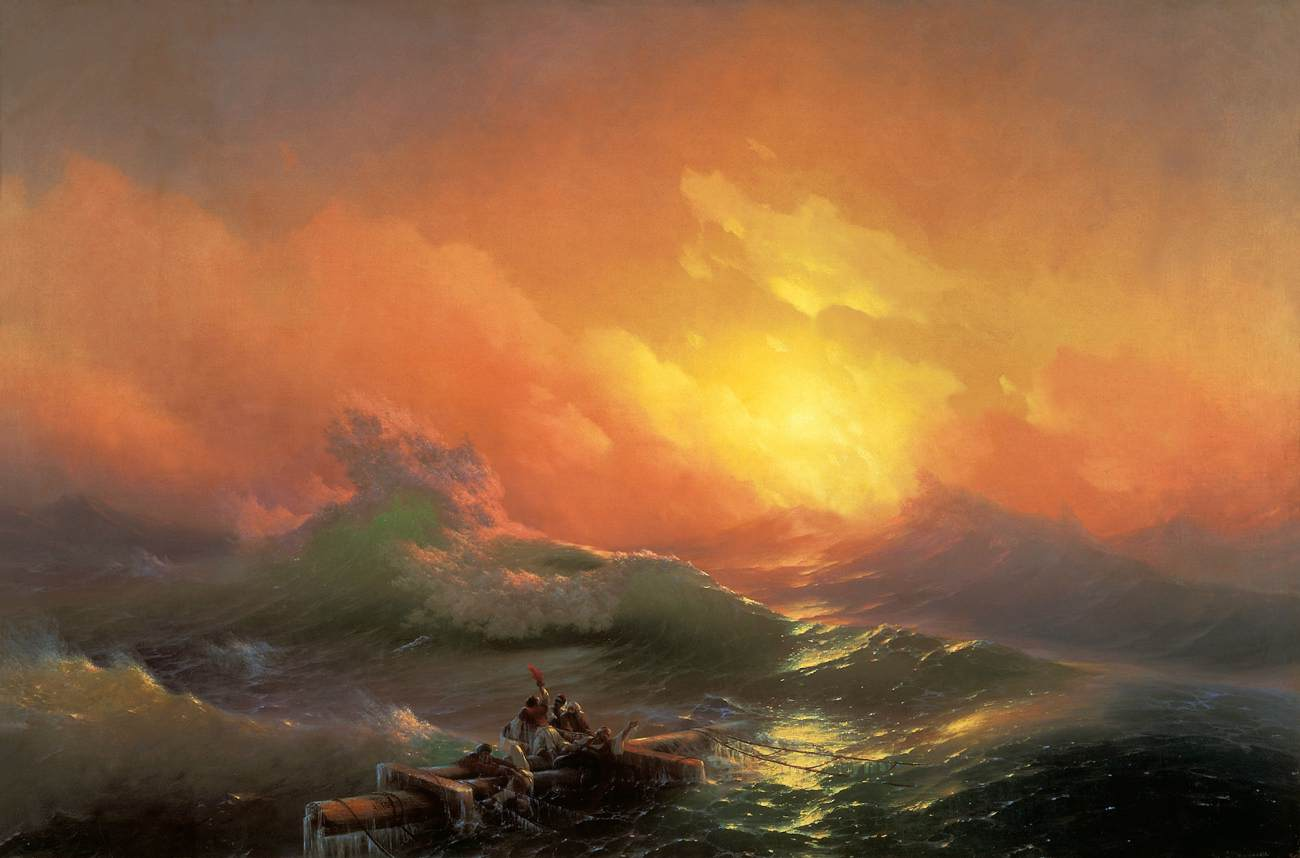
\includegraphics[angle=0,width=0.85\textwidth]{afsnit/afprovning/billeder/thressholds/medium_farver/svage_detalier/sDetalier1.jpg}
        \label{Orginal2}}
        \caption[]{Edgedetection på et billedet med medium farver og få detalier, hvor tærskenværdigern [100,240] er den beste}
     \label{to}
\end{figure}

\begin{figure}[!h]
    \centering
    \subfloat[200,460]{
        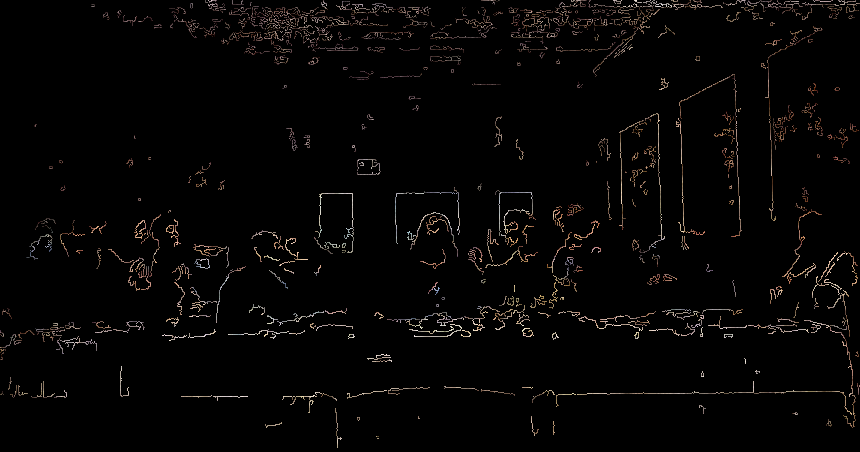
\includegraphics[angle=0,width=0.85\textwidth]{afsnit/afprovning/billeder/thressholds/medium_farver/medium_detalier/2_iteration/200-460.png}
        \label{200-460}}\\
    \subfloat[Orginal]{
        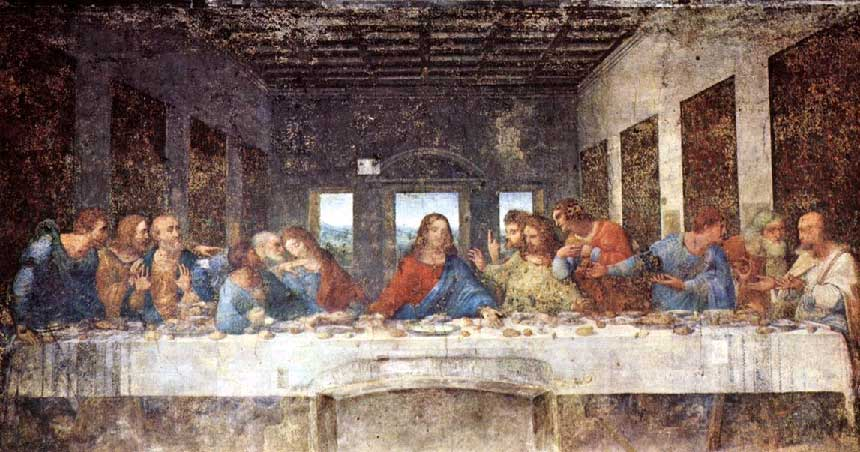
\includegraphics[angle=0,width=0.85\textwidth]{afsnit/afprovning/billeder/thressholds/medium_farver/medium_detalier/mDetalier1.jpg}
        \label{Orginal3}}
        \caption[]{Edgedetection på et billedet med medium farver og medium detalier, hvor tærskenværdigern [200,460] er den beste}
     \label{tre}
\end{figure}

\begin{table}[!h]
    \centering
    \begin{tabular}{| l | l | l | l |} \hline
        & Svage farver 	& Medium farver & Kraftige farver \\ \hline
        Få detalier 		& [100,250]		& [100,240]		& [200,320]\\ \hline
        Medium detalier 	& [100,280]		& [200,460]		& [200,380]\\ \hline
        Mange detalier		& [200,400]		& [200,380]		& [300,750]\\ \hline
    \end{tabular}
    \caption{Beksriv!}
    \label{thressholdsTabelKant}
\end{table}

Som man kan se at tabel \ref{thressholdsTabelKant} gå tærskelværdierne
fra [100,240] til [300,750], så vi kan ikke umiddelbart sætte en fast
tærskelværdi for alle malerier og få at lave en rigtige undersøgelse af
tærskelværdi på malerierne, bliver man nød til at se på mangle flere
malerierne og bestemme deres tærskelværdi og udregne median af de
værdiger, men det vil krave en støre undersøgelse som vi ikke har valt
at gøre, af 3 grunde. 1, det vil kun være en median tærskelværdi få lige
det sæt malerier som vi arbejder på. 2 det vil krave at vi gennemgik
XX(hvor mange) billeder. 3, selv med en median tærskelværdi vil der
stadig være en stor rigge malerier hvor median tærskelværdien ikke vil
være særlige god for. En anden fremgang måde er at regne
tærskelværdierne løbene ud for vært billedet via et program. Men det
problem falder uden for denne opgave og vi vil derfor ikke komme ind på
det. Selv om vi måske ikke kan få det vi helst vil have er der stadig en
del observationer som kan laves ud fra tabellen
\ref{thressholdsTabelKant}. Tærskelværdierne bliver højre nu flere
detaljer og nu kraftigere farverne er. Det virker også som om mange
detaljer vægter lige højt i forholdt til tærskelværdierne en kraftige
farver. Den anden tærskelværdi er ca 2.5 gangen støre en den første
tærskelværdi.

De tærskelværdier som vi har fundet svare til de optimale
tærskelværdier for maleriet, men vi kan godt bruge en værdig som ligger
laver, da metoden floodfill som gør brug af kandtdetektionen resultatset,
god kan tage højde for små kanter, men fejler hvis der ikke er nogle.
Derfor har vi valt at bruger den nederste tærskelværdi som vi har fundet
[100,240] og sænke den lidt til $[78,78 \cdot 2.5 ]$.

\subsection{Afvigelsen af farver i floodfill}
Floodfill har 2 tærskelværdier $lo$ og $up$, som betegner hvor mange pixel
værdier en nabo pixel farver må variere ned og op, en fyldestgørelses
beskrivelse af floodfill findes i afsnit \ref{floodfill}. Vi har tænkt os at
finde en fældes tærskelværdi til brug i vores program. Måde vi gør det på at
ved at observere hvordan floodfill virker med forskellige tærskelværdier og
finde de tærskelværdier som passer bæst til maleriet. Resultatet for
observationen kan ses i tabel \ref{thressholdsTabelFF}, hvor de 9 sammen
kategorier er vist. Et af de malerierne hvor den optimale tærskelværdi er
fundet se i figur \ref{Floodfillbilledet}, så man kan se hvad vi har vurderet
til at være den beste værdi.

\begin{figure}[!h]
    \centering
    \subfloat[8,8]{
        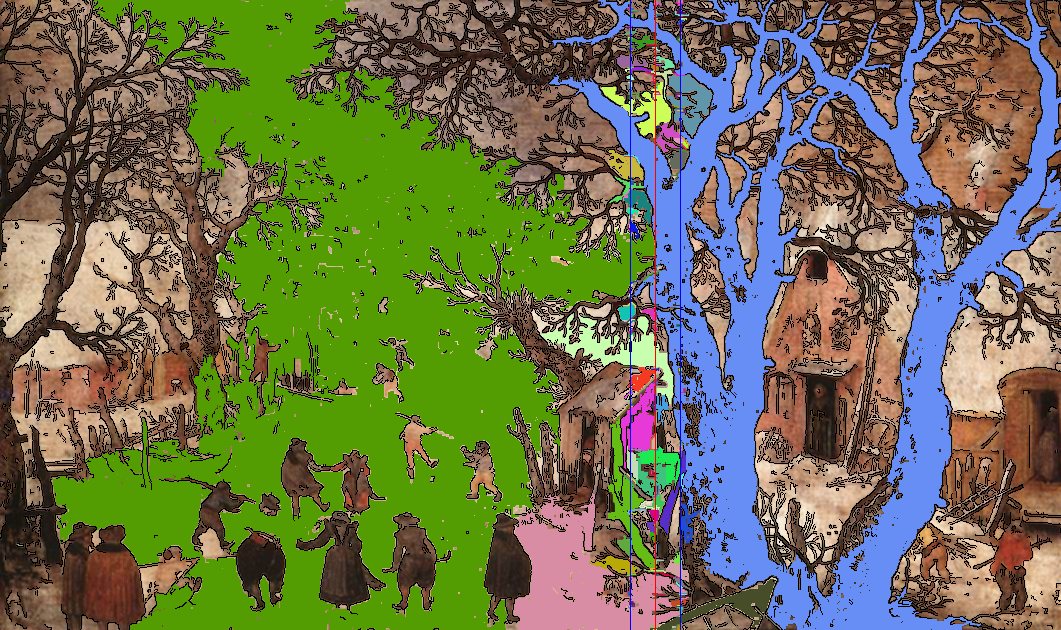
\includegraphics[angle=0,width=0.9\textwidth]{afsnit/afprovning/billeder/thressholds/svage_farver/kraftige_detalier/floodfill/8-8.png}
        \label{8-8}}\\
    \subfloat[Orginal]{
        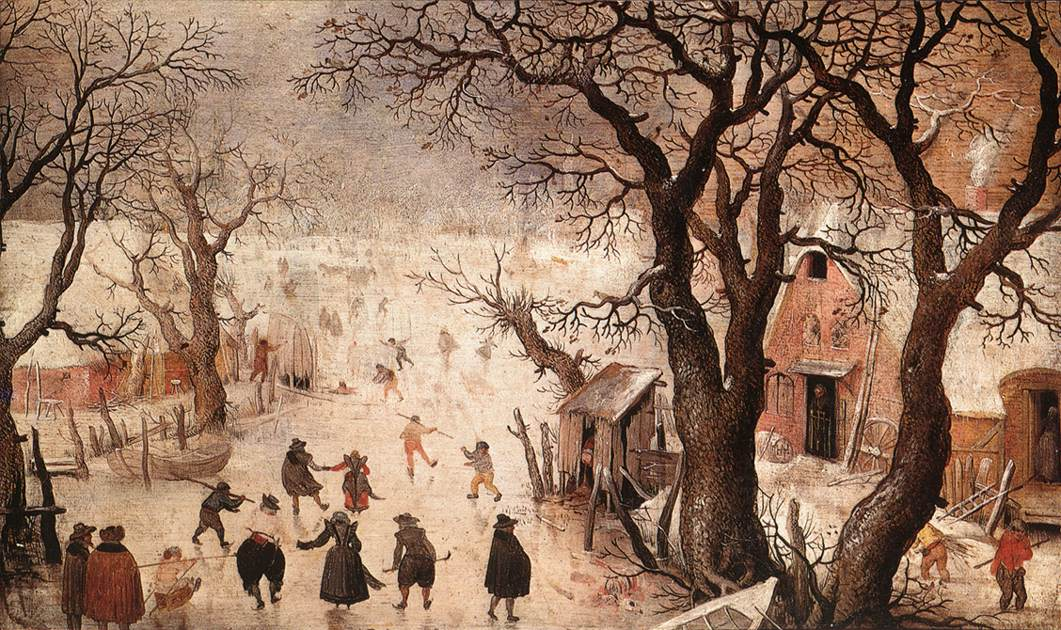
\includegraphics[angle=0,width=0.9\textwidth]{afsnit/afprovning/billeder/thressholds/svage_farver/kraftige_detalier/kDetalier.jpg}
        \label{Orginal4}}
    \caption[]{tærskelværdierne på et billedet med svage farver og kraftige detaljer hvor tærskelværdien [8,8] passer best}
    \label{Floodfillbilledet}
\end{figure}

\begin{table}[!h]
    \centering
    \begin{tabular}{| l | l | l | l |} \hline
        & Svage farver 		& Medium farver & kraftige farver \\ \hline
        Få detalier 		& \textbf{[2,2]}	& [3,3]			& [4,4]\\ \hline
        Medium detalier 	& \textbf{[2,2]}	& \textbf{[5,5]}& \textbf{[2,2]}\\ \hline
        Mange detalier		& [8,8]				& [4,4]			& [7,7]\\ \hline
    \end{tabular}
    \caption{Beskriv!}
    \label{thressholdsTabelFF}
\end{table}

Som man kan af tabellen er nogle af vadierne med fed, begrundelsen for det er
at de vadier er de beste vi kunne finde for billedet, men at de vadier stadig
ikke giver noget som er særlige brugbart, se sektion \ref{floodfilltest}.
værdigerne i tabel fluktuere også en del, så vi har igen samme problem stilling
som i tærskelværdierne ved kantdetektion og har valt at bruge tærskelværdien
[4,4] da dette kommer tættest på gennemsnit.

\section{Regions detektor}
I dette afsnit vil vi afprøve den generelde region detektor, det vil
sige hvad der egentlig bliver fundet inden, vores to metoder sortere
regionerne fra. selve metodes fremgangsmåde er beskravet i sektion
\ref{Sammensetning_af_metoder}, hvor det sideste skrid nå billedet
bliver floodfilldet, derfor vil vi forklare afprøvningen af metode ud
fra billeder som er kommer til dette skridt, hvor tærskelværdierne er
sat til de fundene tærskelværdier. Den første del vil omhandle test på
opbygget billeder og den anden del vil omhandle test på udvalgte
billeder fra vores billedet database.

\subsection{Afprøvning på test billeder}
I dette sektion tester vi på billeder som er konstrueret, men en hvid
baggrund og sorte regioner, det snit vi tester på er indtegnet samt
marginen. I billedet \ref{GRD_test1} er der 5 regioner, hvor 3 af dem bliver
fundet da de ligger i snittet, de 2 regioner som ikke er fundet er
stadig sorte, som man kan se bliver både den er krydser snittet og den
der tangere snittet taget med. I billedet \ref{GRD_test2} er der 3 regioner som
alle bliver fundet, baggrunden, den lille region som ligger inde for
margin, og den store region som kun har en lille del af dens masse inde
i snittet. I billedet \ref{GRD_test3} er der en hoisont som ligger oven på
snittet, begge sider af hoisont linien bliver tegnet med.


\begin{figure}[!h]
    \centering
		\subfloat[4 figure og en bagrun, hvor 2 af figurene og bagrunden er fundet]{
        	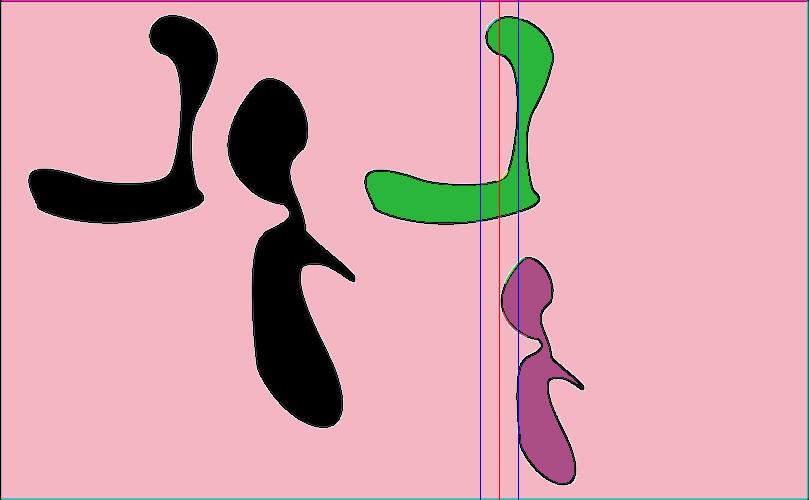
\includegraphics[angle=0,width=0.7\textwidth]{afsnit/afprovning/billeder/region_selector/blob_region_section.png}
        	\label{GRD_test1}}\hspace{1em}
    		\subfloat[En stor figur og en lille figur begge fundet]{
	        	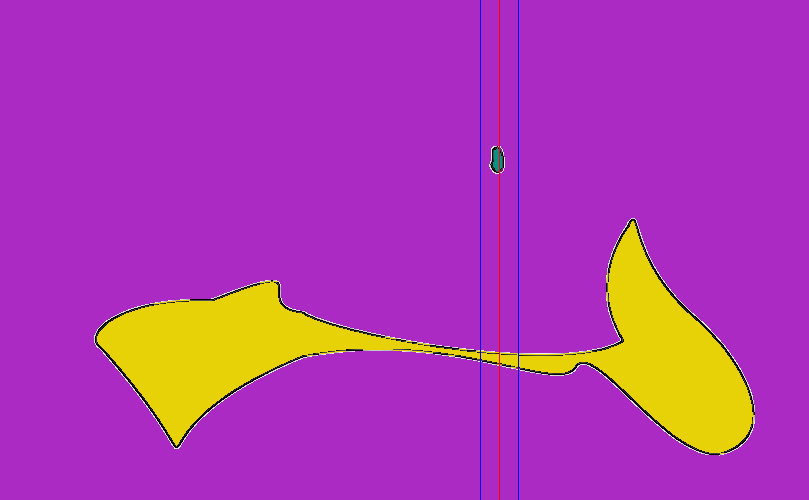
\includegraphics[angle=0,width=0.7\textwidth]{afsnit/afprovning/billeder/region_selector/blob2_region_section.png}
	       	\label{GRD_test2}}\hspace{1em}
    		\subfloat[En hoisont, hvor begge sider er fundet]{
	        	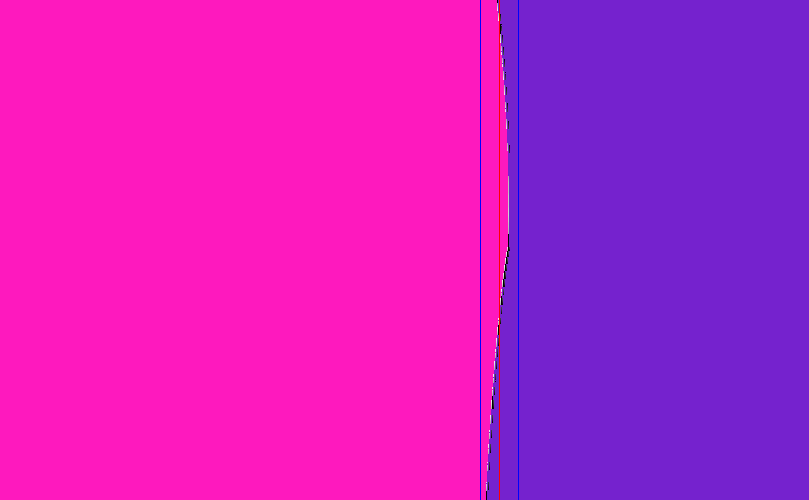
\includegraphics[angle=90,width=0.5\textwidth]{afsnit/afprovning/billeder/region_selector/hoisont_region_section.png}
		       	\label{GRD_test3}}\hspace{1em}
        \caption[]{3 test billeder med bløde former, hvor regien detektor er kørt på dem}
     \label{region_detektor_test}
\end{figure}

I figur \ref{region_detektor_test} er de 3 test billeder afbilledet, de
opføre sig efter de standarter som vi frem satte i afsnit
\ref{}XX(hvilken reference?) 

\subsection{Afprøvning på malerier}
Vi vil afprøve region detektor på 6 udvalte billeder, som vær viser
styrker og svagheder ved region detektoren

\begin{figure}[!h]
    \centering
		\subfloat[Maleri med Kraftige farver og få detaljer]{
        	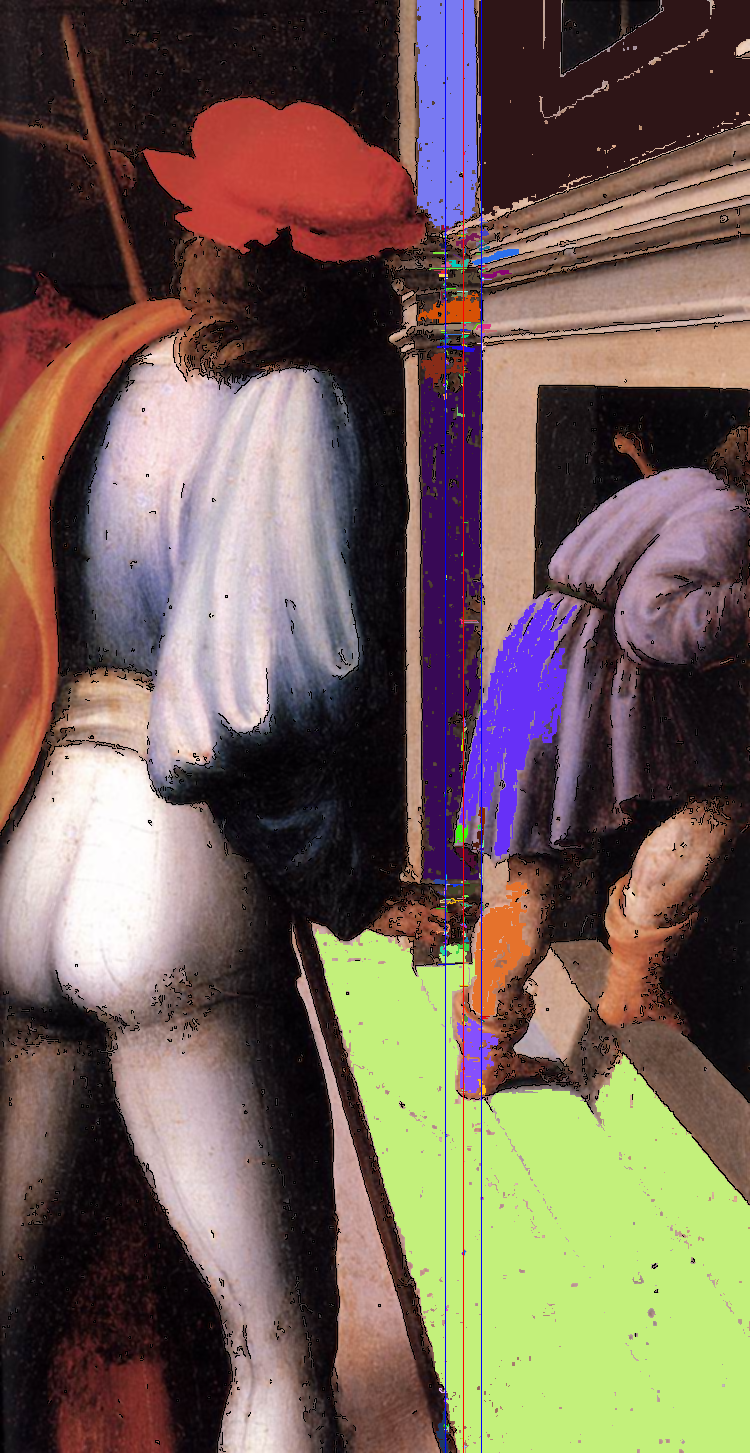
\includegraphics[angle=270,width=1.0\textwidth]{afsnit/afprovning/billeder/thressholds/krafitige_farver/svage_detalier/floodfill/4-4.png}
        	\label{GRD_virker1}}\hspace{1em}
		\subfloat[Medium farver og medium detaljer]{
        	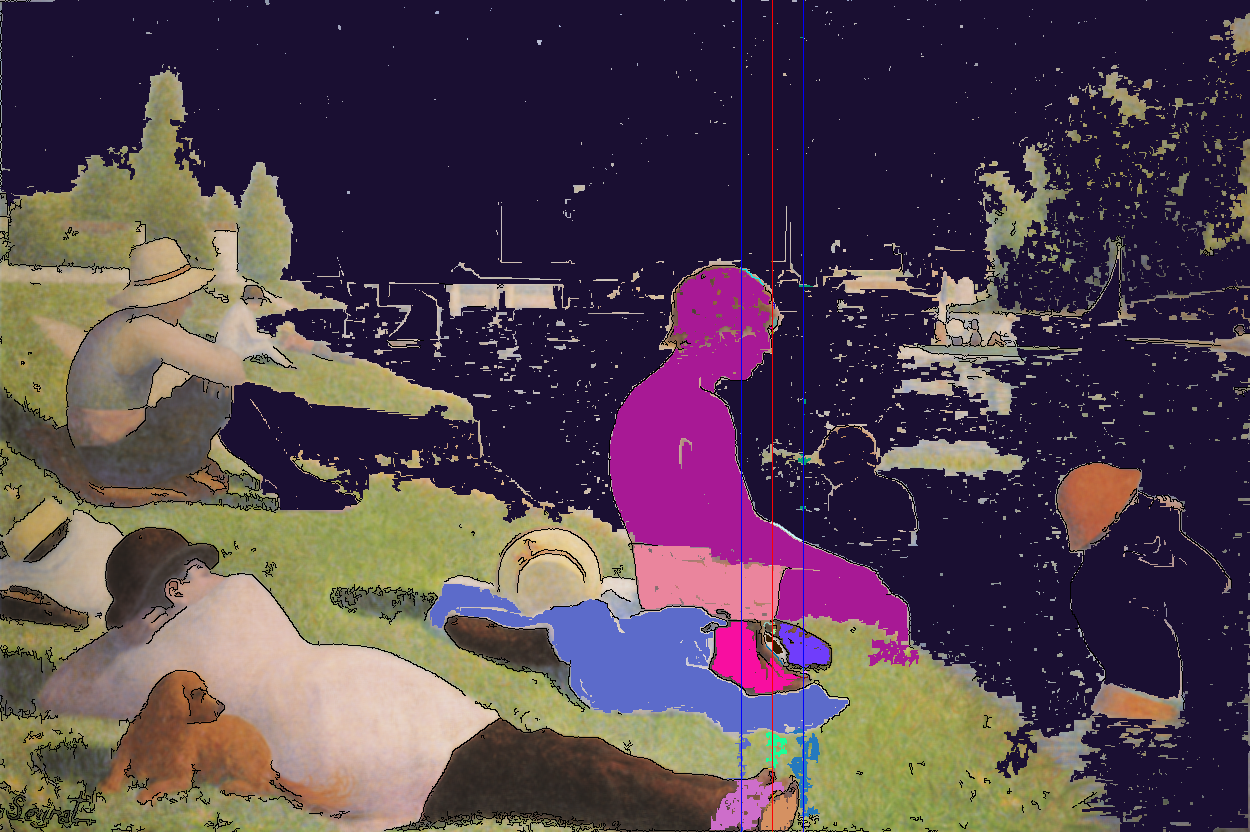
\includegraphics[angle=0,width=1.0\textwidth]{afsnit/afprovning/billeder/4-4.png}
        	\label{GRD_virker2}}\hspace{1em}
        \caption[]{2 malerier hvor regions detektoren virker efter vores ønsker}
     \label{generelde_region_detektor_virker}
\end{figure}

I figuren \ref{generelde_region_detektor_virker} er der 2 malerier, hvor
vores region detektor virker rigtige godt, det første maleri
\ref{GRD_virker1} finder region detektoren 7 store regioner og en masse
små, metoden finder forskel på de forskellige paneler i kaminen og vært
tøj stykke på personen i maleriet er blevet vær deres region, de små
regioner er samlet ved et skift fra et panel til et andet og forstyrrer
ikke de store region ved at gå i gennem dem, man kunne måske have ønsket
at den fylde lidt mere af han karpe ud, men eller et meget godt eksempel
på hvordan den generelde region detektor finde lige det vi vil have den
til at finde. I maleriet \ref{GRD_virker2} finder vi mange af de samme
godt ting, drengen i miden af maleriet er helt udfyldt, en sko og et
håndklæde er også fundet, det er dog vigtigt at ligge mærke til at de
andre personer i vandet, fylder i et med baggrunden, som normalt vil
være en dårlig ting, men som ikke gør noget her da, metoden kun ser
efter regioner i snittet, repræsenteret af den røde linie.
 
\begin{figure}[!h]
    \centering
		\subfloat[Kraftige farver og mange detaljer]{
       	 	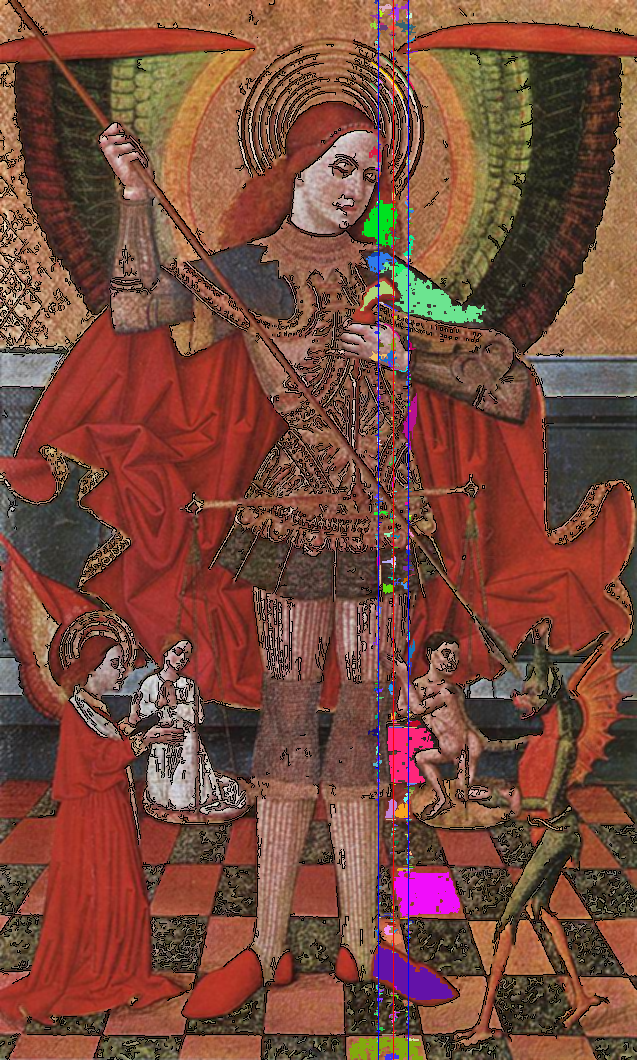
\includegraphics[angle=270,width=0.90\textwidth]{afsnit/afprovning/billeder/thressholds/krafitige_farver/krafite_detalier/floodfill/4-4.png}
		    \label{GRD_virker_nesten1}}\hspace{1em}
    \subfloat[Medium farver og medium detaljer]{
        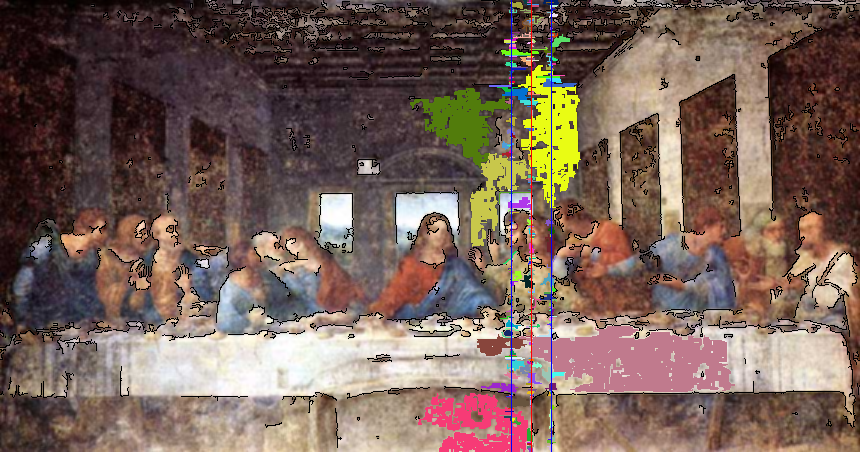
\includegraphics[angle=0,width=0.95\textwidth]{afsnit/afprovning/billeder/thressholds/medium_farver/medium_detalier/floodfill/4-4.png}
        \label{GRD_virker_næsten2}}\\
     \label{generelde_region_detektor_virker_nesten}
     \caption[]{2 malerier hvor regions detektoren ikke helt virker efter vores ønsker men stadig har noget vi kan bruge}
\end{figure}

I figuren \ref{generelde_region_detektor_virker_nesten} er der 2
malerier, hvor vores region detektor ikke virker efter vores ønsker med
stadig har noget vi kan bruge, I maleriet \ref{GRD_virker_nesten1}
bliver der mest fundet små region dog bliver en sko, en skulder og en
flise fundet, hvor vi gerne vil have at personens karpe og arm også blev
fundet, dette skyldes primert at tærskelværdierne for dette billedet er
sat for lavt. Det andet maleri \ref{GRD_virker_nesten2} har nogle af de
samme problematiker, region detektoren finder mest en masse små stykker
af noget som burde hænge sammen. Det vil også kunne løses ved nogle
andre tærskelværdier, men som man også kan se på maleriet er væge og
loftet som egentlige er ret ensfarvet stadig svære for vores region
detektor at fange, det tyder på at en støre sløring godt kunne være
problemløseren få at algoritmen virker på dette maleri. Grunden til at
lige de her 2 bilder er interessante er at ved ændring på tærskelværdier
og sløring kunne vores region detektor virker godt XX(her skal der
billeder hvor det virker), 

\begin{figure}[!h]
    \centering
    \subfloat[Kraftige farver og medium detaljer]{
        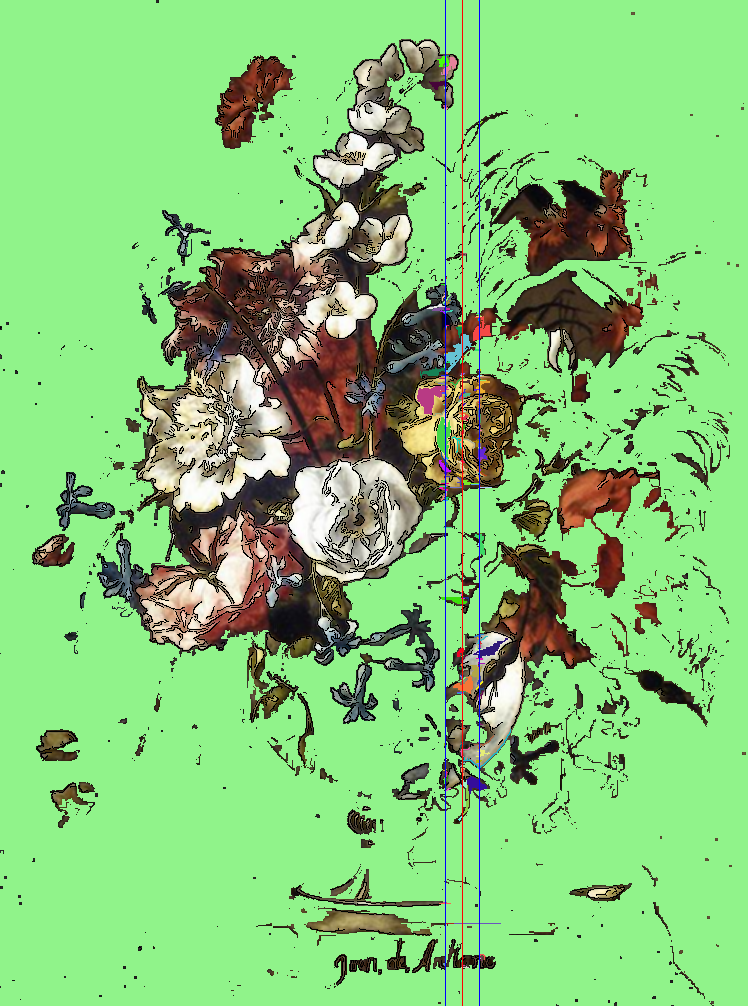
\includegraphics[angle=0,width=0.65\textwidth]{afsnit/afprovning/billeder/thressholds/krafitige_farver/medium_detalier/floodfill/4-4.png}
        \label{GRD_virker_ikke1}}\\
    \subfloat[Svage farver og få detaljer]{
        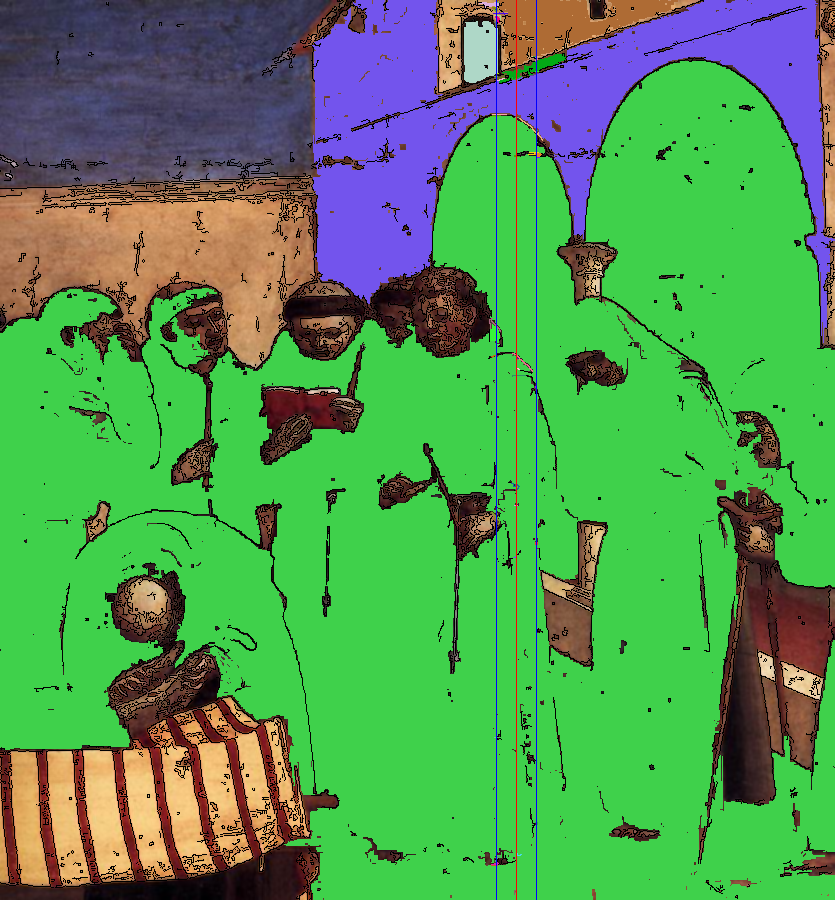
\includegraphics[angle=0,width=0.65\textwidth]{afsnit/afprovning/billeder/thressholds/svage_farver/svage_detalier/floodfill/4-4.png}
        \label{GRD_virker_ikke2}}\hspace{1em}
     \label{generelde_region_detektor_virker_ikke}
\end{figure}

I figur \ref{generelde_region_detektor_virker_ikke} er der 2 malerier
hvor vores region detektor ikke virker særlige godt. I maleri
\ref{GRD_virker_ikke1} er noget af buketten og baggrunden gået i et. På
samme tid er resten af blomsterne i snittet ikke fyldt ud, og selv med
en ændring i tærskelværdierne vil det ikke hjælpe, da en øgning af
tærskelværdierne vil resultere i at flere af blomsterne gå i et med
baggrunden, og en sænkning, vil resultere i at ingen af blomsterne vil
blive detektet. Maleriet \ref{GRD_virker_ikke2} har en anden
problemstiling som vi ikke kan komme uden om, farverne er så mørke og
svage at en ændring i tærskelværdien i floodfill på bare 1 vil få
regiondetektoren til at gå fra at finde ingen regioner til at finde en
stor, som på billedet, dette kan også skyldes at kantdetektionen
tilføje en mørk kan rundt om regionerne, men da maleriet er mørkt i
forvejen hjælper kandetektionen ikke.
XX(jeg kan ikke helt prolamere dette unden at have nogle bileder at bagge det op)


\section{Naive løsning}
%% Bemærk:
%%          Resten af rapporten følger en stil hvor indledninger skrives
%%          med \sffamlily-typen. Denne stil bør også følges her.
%%
{\sffamily
I dette sektion vil vi teste den naive løsning. ved at se om den sortere
de rigtige regioner væk og om løsningen opføre sig på samme måde som vi
har håbet på. Det vil vi gøre ved ført at se på nogle fabrikeret test
billeder, får at se om den naive løsning virker efter meningen og
bagefter vil vi teste på malerierne for at se om den naive løsning kan
bruges i praktisk.
}
  
\subsection{Afprøvning på testbilleder}
Vi vil teste på de samme testbilleder som i sideste afsnit, samt et nyt
testbilleder som blev brugt i forklaringen af den naive metodes, de fire
billeder som vi har valt at test kan se i afsnit \ref{region_detektor}
og billedet \ref{naiv_masse_original} hvor en grån kasse rundt om en
region, betyder at den er valt til at ligge i det gyldne snit af den
naive metode. 

Det første billedet \ref{naiv_blob1}, har fem regioner og hvor tre af
dem blev fundet af reginon detektoren, vores naive løsning har så
sorteret baggrundens regionen og den øverste region i snitte vær, da de
begge krydser marginer og derfor ikke overholder definition
\ref{} . 

\begin{figure}[!h]
	\begin{center}
        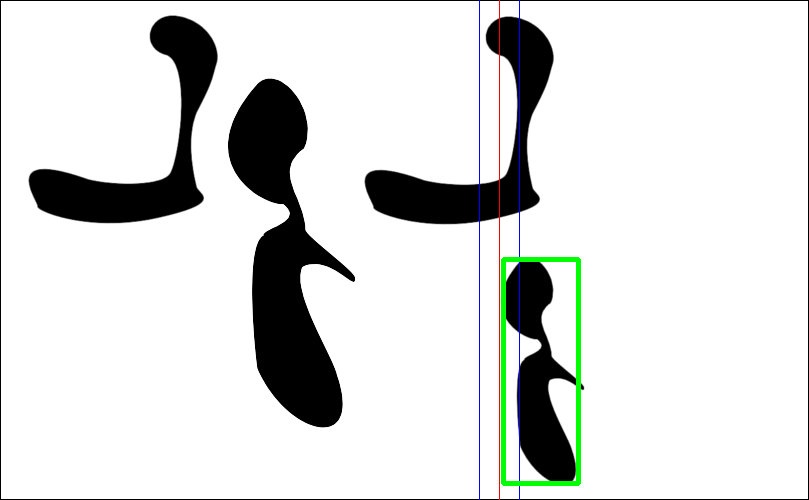
\includegraphics[angle=0,width=0.55\textwidth]{afsnit/afprovning/billeder/naive_losning/naiv_blob1.png}
	\end{center}       
	\caption{Naive algoritme finder en ud af fem regioner}	
	\label{naiv_blob1}
\end{figure}

Det andet billedet \ref{naiv_blob2}, er alle blevet sorteret vær, også
den lille, da den er for lille, derfor ikke overholder definition
\ref{def_interessant} b. 

\begin{figure}[!h]
	\begin{center}
       	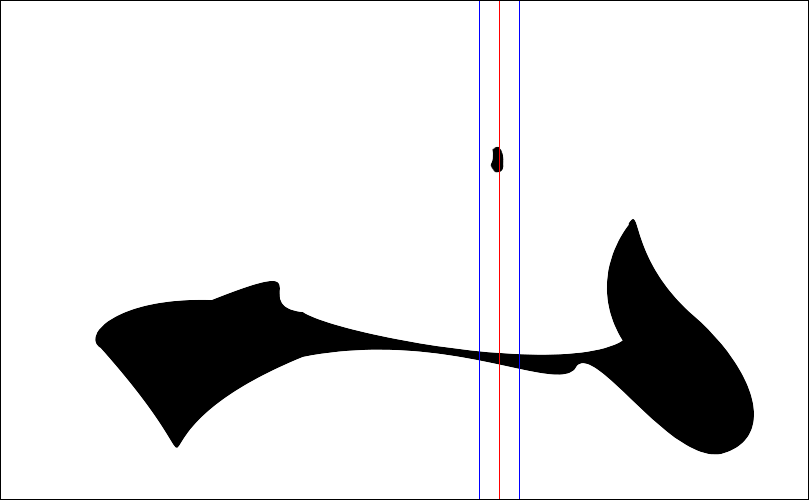
\includegraphics[angle=0,width=0.55\textwidth]{afsnit/afprovning/billeder/naive_losning/naiv_blob2.png}
	\end{center}
	\caption{Værgen den lille region eller den store er fundet} 
   	\label{naiv_blob2}
\end{figure}

I test billedet \ref{naive_hoisont1}, sortere algoritmen
himlen fra, da den krydser margin lidt, men tager jorden med. 

\begin{figure}[!h]
	\begin{center}
       	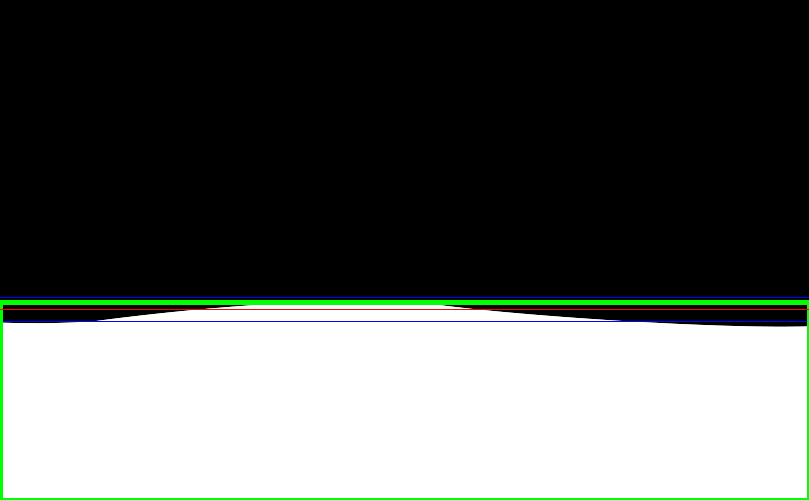
\includegraphics[angle=0,width=0.55\textwidth]{afsnit/afprovning/billeder/naive_losning/naiv_hoisont1.png}
	\end{center}
	\caption{Kun den nederste højrisondt er fundet} 
   	\label{naive_hoisont1}
\end{figure}

\clearpage

\subsection{Afprøvning på malerier}
Vi afprøver den naive algoritme på seks malerier, først på tre malerier,
hvor regions detektoren virker efter vores hensigt og så på ter
malerier, hvor region detektoren ikke virker. Beskrivelsen af hvad der
sker i billedet vil står i caption


\begin{figure}[h!!]
	\begin{center}
		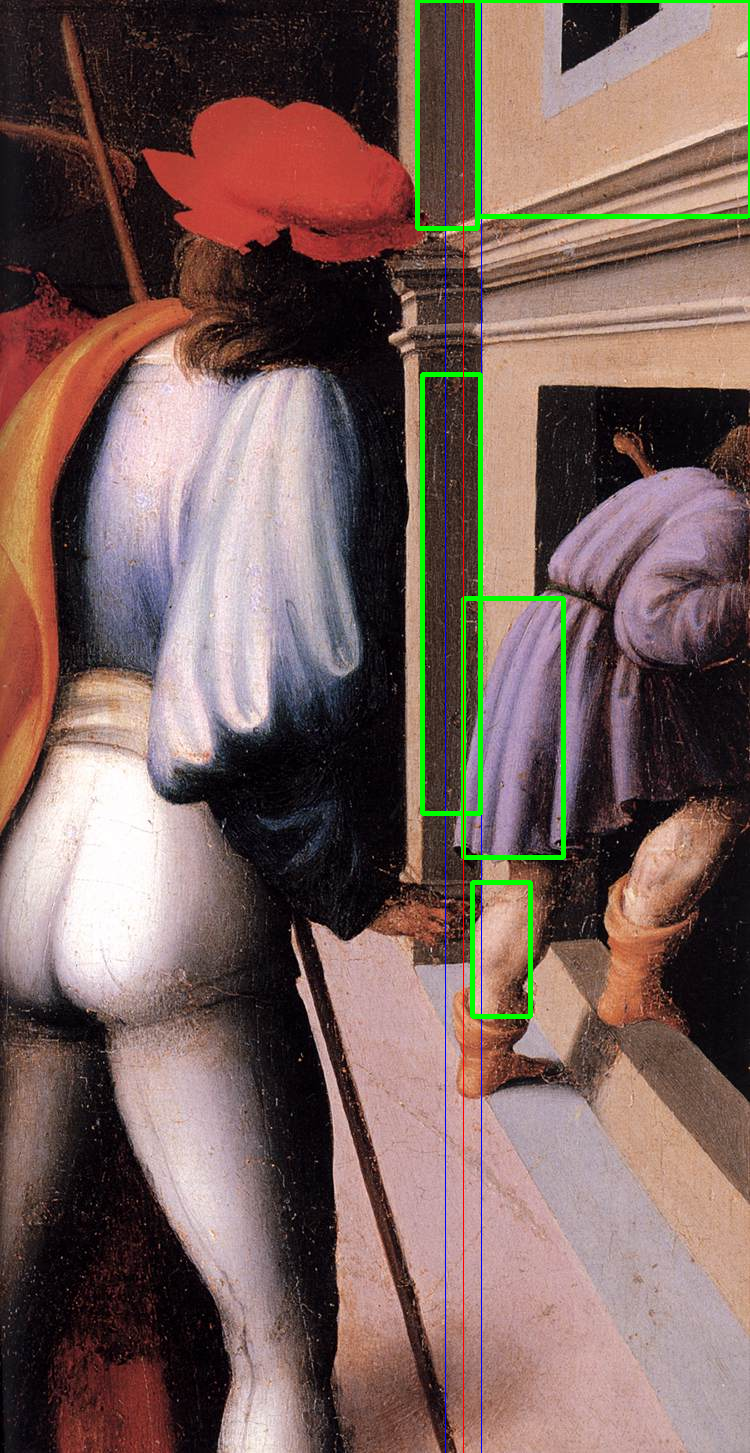
\includegraphics[scale=0.3,angle=0]{afsnit/afprovning/billeder/naive_losning/naiv_kfarver_sdetaljer.png}
	\end{center}
	\caption[]{Fem ud af de seks store regioner fra figur
	\ref{GRD_virker1} valt til at ligge i snittet, skoene er få små til
	at blive taget i betragtning}
	\label{naiv_kfarver_sdetaljer}
\end{figure}

\begin{figure}[h!!]
	\begin{center}
		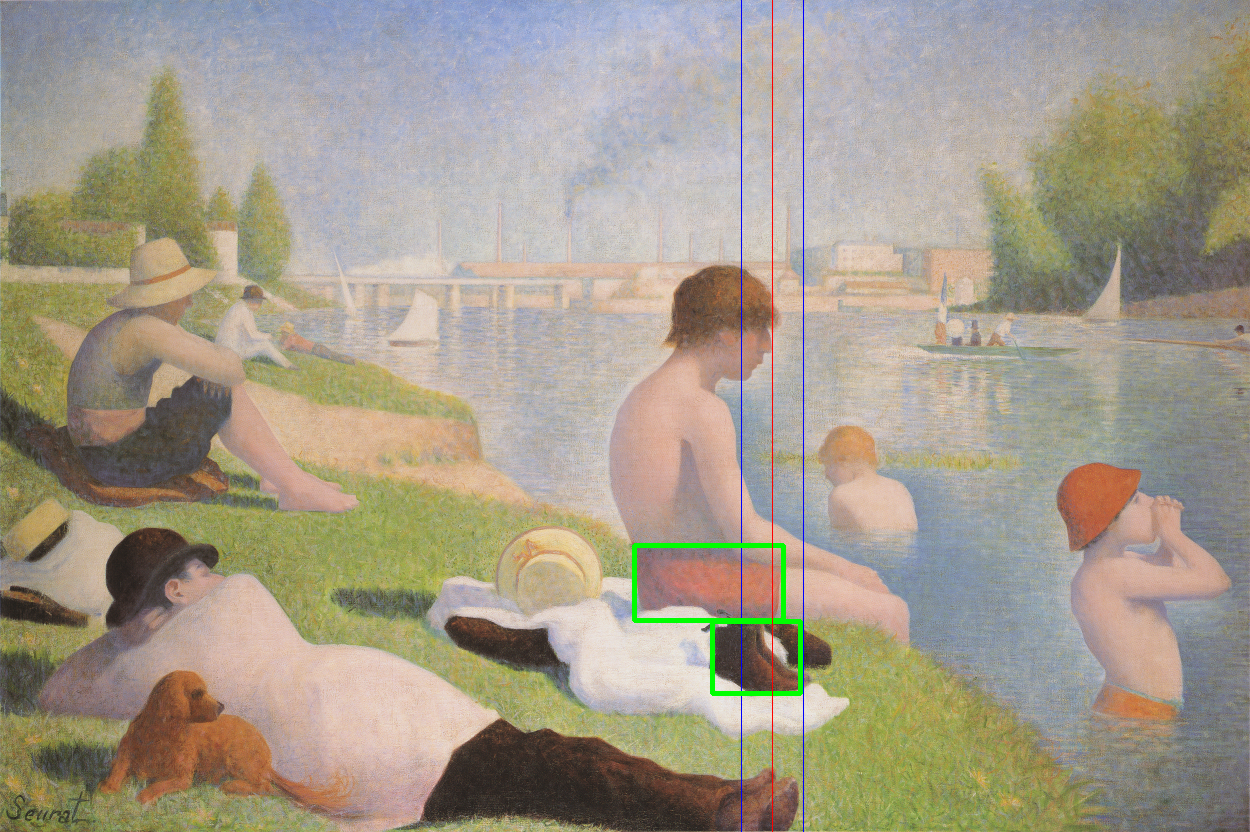
\includegraphics[scale=0.3,angle=0]{afsnit/afprovning/billeder/naive_losning/naiv_mfarver_mdetaljer.png}
	\end{center}
	\caption[]{Bukserne og skoene er tager med af den naive løsning, men
	drengen er sorteret væk da har krydser snittet}
	\label{naiv_mfarver_mdetaljer}
\end{figure}

\begin{figure}[h!!]
	\begin{center}
		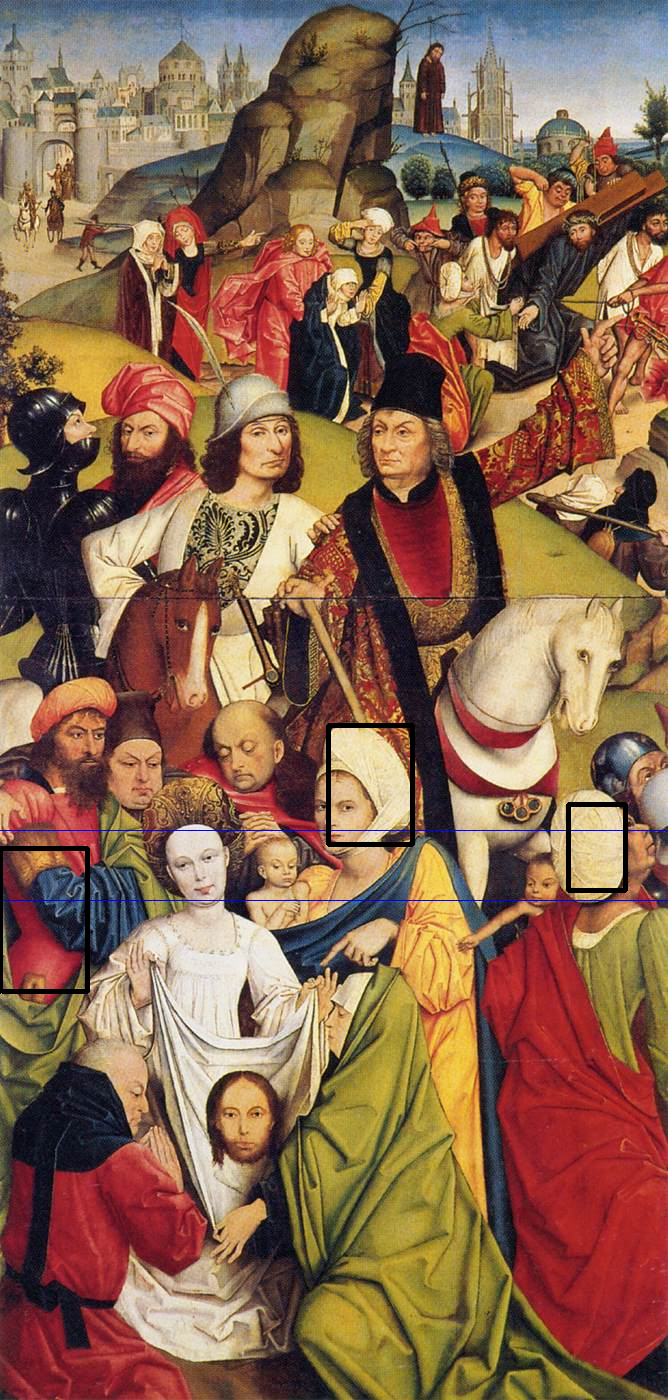
\includegraphics[scale=0.3,angle=0]{afsnit/afprovning/billeder/naive_losning/naiv_kfarver_kdetaljer.png}
	\end{center}
	\caption[]{Et billedet med mange hoder i snittet, hvor to af dem
	bliver godtaget af den naive metode til at ligger i snittet, en
	trøje bliver desværre også taget med. Navn: Christ Carrying the
	Cross. År: 1480. Af: Bosch Hieronymus}
	\label{naiv_kfarver_kdetaljer}
\end{figure}

\begin{figure}[h!!]
	\begin{center}
		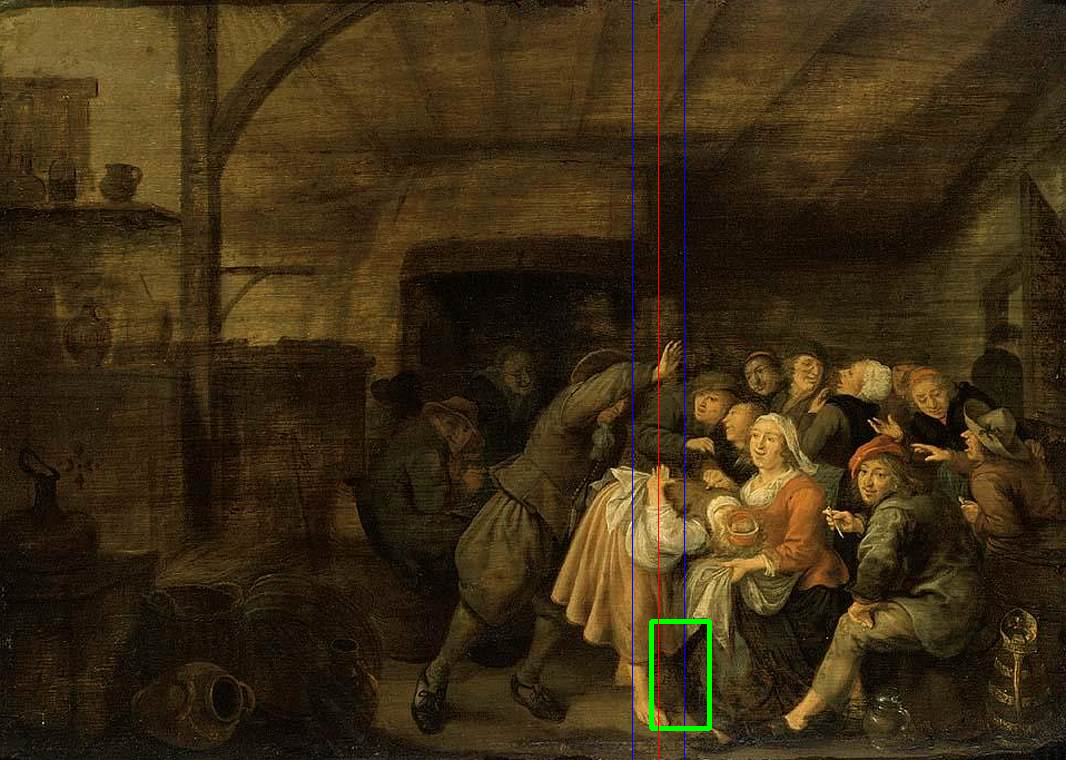
\includegraphics[scale=0.3,angle=0]{afsnit/afprovning/billeder/naive_losning/naiv_virker_ikke1.png}
	\end{center}
	\caption[]{Mallerie hvor region detektor ikke virker, den naive
	løsning godtager tager en region som ligger helt forkert. Navn:
	Peasants in an Inn Playing "La Main Chaude". År: Ukendt. Af:
	Molenaer, Jan Miense.}
	\label{naiv_virker_ikke1}
\end{figure}

\begin{figure}[h!!]
	\begin{center}
		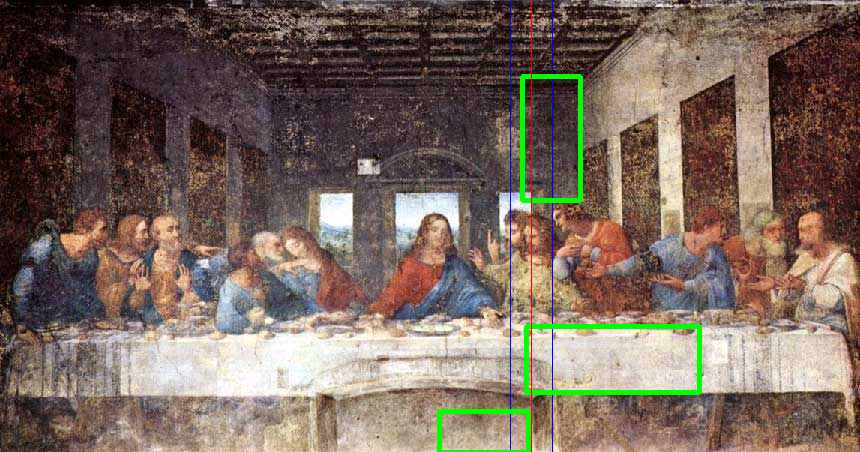
\includegraphics[scale=0.3,angle=0]{afsnit/afprovning/billeder/naive_losning/naiv_virker_ikke2.png}
	\end{center}
	\caption[]{Tre regioner bliver godtaget, selv om de ikke er særlige
	intresante }
	\label{naiv_virker_ikke2}
\end{figure}

\begin{figure}[h!!]
	\begin{center}
		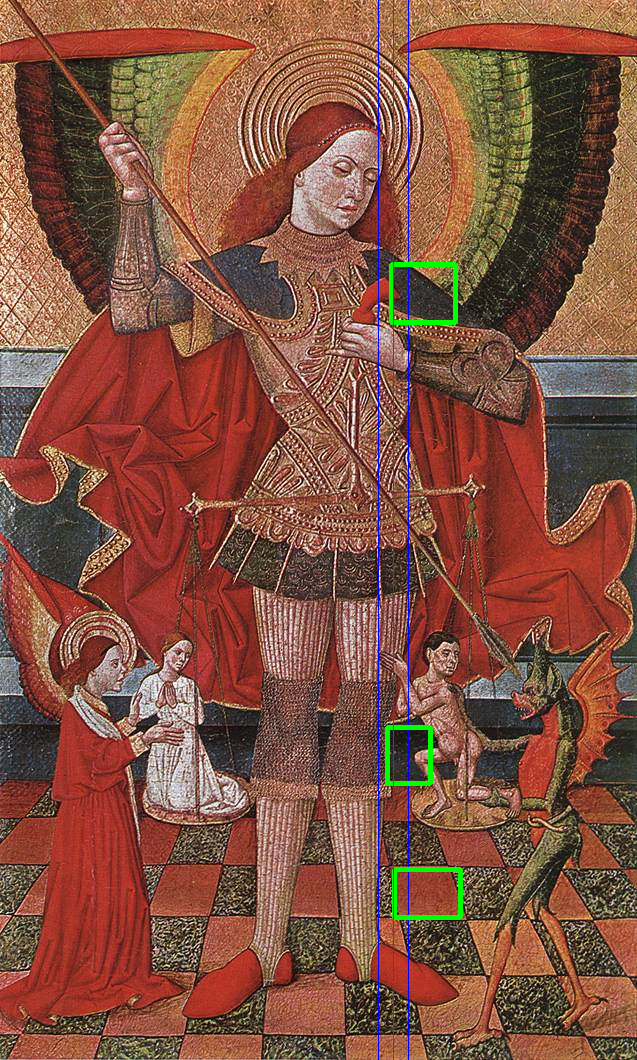
\includegraphics[scale=0.3,angle=0]{afsnit/afprovning/billeder/naive_losning/naiv_virker_ikke3.png}
	\end{center}
	\caption[]{Der bliver fundet tre region, hvor kun en af dem passer
	på en ting i billedet}
	\label{naiv_virker_ikke3}
\end{figure}
\clearpage

\subsection{Konkulution}
Det virker som om den naive løsning virker efter vores entationer dog
med nogle få falske positive, hvis region detektoren virker på
malerierne, dog fejler den på malerier hvor region detektoren fejler, og
kommer med en masse falske positive.

\section{Udvidet løsning}


}

% vim: set tw=72 spell spelllang=da:


\chapter{Videnskabelige resultater}

% sort in citation order
\bibliographystyle{unsrt}
\bibliography{litteraturliste}
\addcontentsline{toc}{chapter}{Litteratur}

\chapter{Bilag}
\appendix

%\section{Kildekode}
%\input{materialer.tex}
%\newpage

\end{document}
